\documentclass[../thesis.tex]{subfiles}
% !TeX spellcheck = fr_FR

\begin{document}
    \chapter{Introduction}
    \label{chap:Introduction}
    \setcounter{page}{1}
    %\vfill
    %\begin{figure}[H]
    %	\centering
    %	\includegraphics[width=0.7\linewidth]{img/00-cover-semeuses}
    %	\caption*{Les Semeuses 1857}
    %\end{figure}
    
    Ce chapitre présente les principaux modèles de production agricole et leurs évolutions. Il aborde dans une première partie les intérêts et limites de l'agriculture conventionnelle. Dans une seconde partie, il s'intéresse à la transition agroécologique et à l'agriculture de précision. L'intérêt des systèmes d'imagerie et des méthodes de traitement des données numériques sera notamment souligné.
    %\vfill
    
    %\newpage
    
    
    \section{Agriculture : un avènement}
    
    %! C.Gée
    %\par L'avènement de l'agriculture a été un moment décisif pour l'humanité. Le développement des pratiques agricoles est une histoire qui a évolué au cours de millier d'années. La première période de grands changements remonte à la moitié du XXème siècle où l'agriculture s'est considérablement modernisée, passant d'une agriculture traditionnelle à une agriculture mécanisée, grâce à l'essor des sciences et techniques telles que la mécanique, l'hydraulique et l'électrotechnique.	Cette période d'environ 50 ans marque donc le début de l' accélération démographique, de la consommation d'eau et d'énergie. C'est l'anthropocène (figure \ref{fig:02-anthropocène}) caractériser par l'ensemble des événements géologiques qui se sont produits depuis que les activités humaines ont une incidence globale significative sur l'écosystème terrestre.
    
    %! JNP
    %\par Apparue au Néolithique, l'agriculture a constamment évoluée tout au long de l'histoire de l'humanité. Le XXe siècle a été marqué par des changements rapides et par des gains de productivité importants, principalement liés au développement de la mécanisation, et à l'utilisation d'intrants de synthèse (engrais chimiques et produits phyto-pharmaceutiques). Ces changements s'inscrivent dans un contexte global d'accélération de la démographie, et de la consommation des ressources naturelles. C'est l'Anthropocène (figure \ref{fig:02-anthropocène}) caractérisé par l'ensemble des événements géologiques qui se sont produits depuis que les activités humaines ont une incidence globale significative sur l'écosystème terrestre.
    
    %! Mehdi
    \par Apparue au Néolithique, l'agriculture a constamment évolué tout au long de l'histoire de l'humanité. Les premiers grands changements remontent à la moitié du XXe siècle où l'agriculture s'est considérablement modernisée. En effet, l'agriculture traditionnelle évolue vers une agriculture mécanisée grâce à l'essor des sciences et techniques telles que la mécanique, l'hydraulique et l'électrotechnique. Cette période s'inscrit dans un contexte global d'accélération de la démographie et de la consommation des ressources naturelles, c'est l'Anthropocène \cite{federau2016philosophie}. Elle est caractérisée par l'ensemble des événements géologiques qui se sont produits depuis que les activités humaines ont une incidence globale significative sur l'écosystème terrestre.
    %perrier2013anthropocene
    
    \begin{figure}[H]
        \centering
        \rotatebox{90}{\scriptsize (source: \href{https://sciences-critiques.fr/allons-nous-vraiment-entrer-dans-lanthropocene/}{sciences-critiques.fr})}
        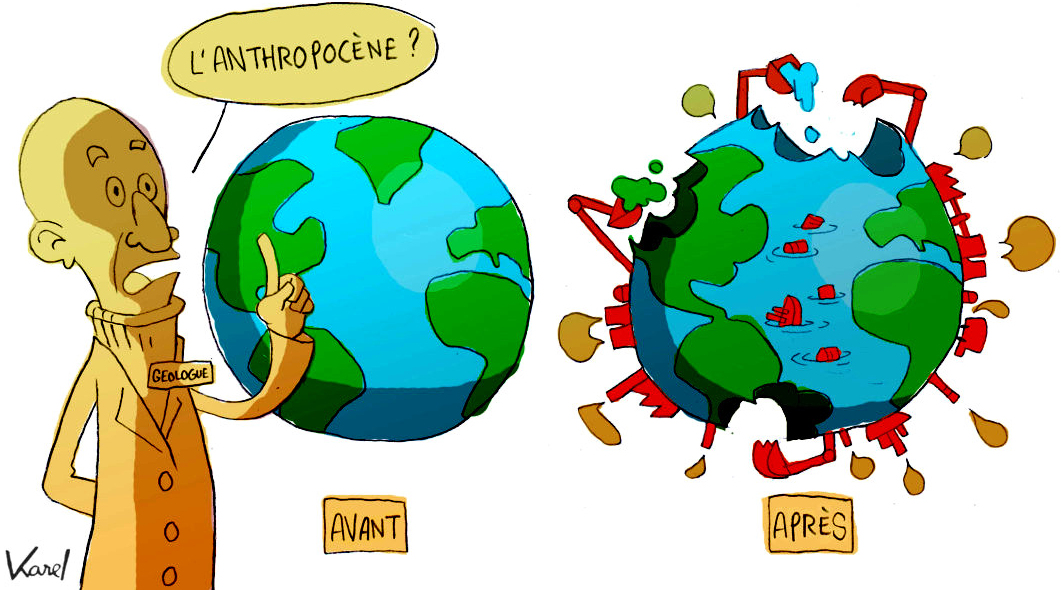
\includegraphics[width=0.4\linewidth]{./img/intro/intro-anthropocene.jpg}
        \caption{L'Anthropocène}
        \label{fig:02-anthropocène}
    \end{figure}
    
    %!JNP
    %\par La production agricole a été fortement accrue, mais le modèle actuel, l'agriculture conventionnelle, soulève de nombreuses questions relatives à sa viabilité économique (prix de vente des productions, coût des intrants), à son impact sur la santé des consommateurs (qualités nutritionnelles des produits, résidus de pesticides) et à son empreinte environnementale (changement climatique, baisse de la biodiversité). La baisse des prix a également engendrée des conséquences sociales importantes, avec une baisse significative du nombre d'exploitants à travers le monde, ayant des salaires très faibles (suicide, non-reprise, \dots \cite{chaumeil1939travaux, shiva2006seeds, carles2007volem, nagaraj2008farmers, Suicide2021, utyasheva2021suicide}), passant donc d'une agriculture rurale à une production industriel. % et diversifié à la mécanisation via le grand remembrement de terre agricoles.
    
    La production agricole a été fortement accrue, mais le modèle actuel (i.e l'agriculture conventionnelle), soulève de nombreuses questions relatives à sa viabilité économique (prix de vente des productions, coût des intrants), à son impact sur la santé des consommateurs (qualités nutritionnelles des produits, résidus de pesticides) et à son empreinte environnementale \cite{loiret:tel-01306180} (changement climatique, baisse de la biodiversité). La baisse des prix a également engendré une chute des salaires engendrant des conséquences sociales importantes, avec une baisse significative du nombre d'exploitants à travers le monde (suicide, non-reprise, \dots) \cite{chaumeil1939travaux, shiva2006seeds, carles2007volem, nagaraj2008farmers, Suicide2021, utyasheva2021suicide}. Dans un souci d'augmenter la production, l'agriculture rurale évolue ainsi vers une production industrielle.
    
    %! C.Gée
    %\par Cette mécanisation a permis à la France de rendre sa production agricole exportatrice. De plus, l'avènement de « la chimie de synthèse » a conforté cet élan de productivité, dopant les rendements avec l'utilisation d'engrais chimiques et de produits phyto-pharmaceutiques : l'agriculture française ``rayonne''. Le double choc pétrolier de 1975 et 1979 enclenche une augmentation drastique du coût de ces produits de synthèse. De plus, la disparition des montants compensatoire en Europe n'est pas sans conséquence sur les performances économiques des exploitations agricoles (seul critère d'évaluation pris en compte). S'engage alors dans les années 1980 de nombreuses réflexions. Certes, les rendements ont été multiplié par 3-4. Certes, ils ont permis la baisse des prix pour les consommateurs. Cependant, leurs effets ont aussi engendrés des conséquences importantes d'un point de vue économique, qualitatif, nutritionnelle et environnemental. L'usage de pesticide à été multiplié par 25 engendrent un appauvrissement significatif de la bio-diversité. De plus la baisse des prix a également engendrée des conséquences sociales importantes, avec une baisse significative du nombre d'exploitants ayant des salaires très faibles (suicide, non-reprise, \dots \cite{chaumeil1939travaux, shiva2006seeds, carles2007volem, nagaraj2008farmers}), passant donc d'une agriculture rurale et diversifié à la mécanisation via le grand remembrement de terre agricoles.
    
    %! Au delà du discours politique, sur le côté purement terrain, un système \SI{100}{\percent} artificiel type tomate bio sous serre n'a pas de problème de productivité.
    %! C'est juste une question de dimensionnement de l'exploitation.
    %! C'est seulement si tu veux arrêter l'artificialisation que tu as besoin de la MO et de la vie organique du sol
    
    %! C.Gée
    %\par Pour autant, bien que l'apport de l'agriculture a été indispensable aux développements de nos sociétés modernes, sont essor a pris un tournant décisif cette dernière décennie. Avec la mécanisation en 1950 et l'adoption de la Politique Agricole Commune (PAC), ratifiée en 1962 visant à accroître la productivité de l'agriculture et les bénéfices sans limite dans le temps, le système agricole européen s'enraye en s'engageant dans un processus de destruction de la bio-diversité \cite{diamond2010worst, alma991008709229705596}. Le changement climatique, le potentiel génétique des cultures, les réponses politiques, le cout énergétique, le manque d'environnement favorable, le manque de capacité d'investissement des agriculteurs, la micro et macro-économie sont autant de facteurs qui empêche de revenir immédiatement sur un système de services écosystèmiques. Pour mieux comprendre la situation actuelle de notre agriculture et de l'écologie, il faut s'intéresser aux limites et vulnérabilités des systèmes complexes lié à la dynamique des systèmes \cite{radzicki2008origin} et essayer dans apporter des solutions en revenant aux fondamentaux de l'agronomie et de l'écologie, à travers l'agroécologie et en prenant en compte l'émergence d'une agriculture de précision. L'agriculture de précision est un axe permettant cette transition.
    
    %! JNP
    Les solutions étudiées visent à réduire les quantités globales d'intrants employées, et à en éliminer certains. La suite de ce chapitre s'intéresse aux scénarios d'évolution de notre écosystème et à la manière dont ils sont pris en compte par nos politiques publiques. Il détaille ensuite les modes de production usuels, puis s'intéresse aux limites de l'agriculture intensive et à la transition agroécologique. 
    
    %! Un système artificiel et chimique, il y a corrélation mais pas causalité avec l'enraillement de l'agriculture et la chute de la BioD.
    %! l'agriculture des américains n'est pas enraillée. Si elle l'est c'est plus à cause du changement climatique que de la disparition de la BioD qu'ils flinguent au napalm.
    %! Si le système français s'enraille, c'e.st pour deux choses : le changement climatique et le potentiel génétique des plantes atteints.
    %! Ça ne serait pas gênant si les exploitations avaient des capacités d'adaptation
    %! En fait c'est plus un problème de limite macro et micro économiques des modèles français
    %! Et parallèlement à ça, la BioD a foutu le camp, ce qui empêche de revenir immédiatement sur un système de services écosystèmiques.
    %! L'agroécologie n'est possible pour les agriculteurs qu'avec de la capacité d'investissement. 
    %! Il faudra donc mettre le hola sur la volatilité du marché des commodities
    
    % L'agriculture française est enrayée pcq ils n'ont plus assez d'environnement favorable ni de capacité d'investissement pour que l'agroécologie fonctionne pour le plus grand nombre.
    
    \newpage
    \subsection{Dynamique des systèmes}
    
    La dynamique des systèmes est une approche pour comprendre le comportement des systèmes complexes dans le temps \cite{ArthurKeller}. Cette approche peut être utilisée par exemple pour modéliser les limites et vulnérabilités de notre système de production agricole. Pour cela, deux facteurs biophysiques sont utilisés :
    %La dynamique des systèmes est une approche pour comprendre le comportement des systèmes complexes dans le temps. Cette approche peut être utilisée par exemple pour modéliser les limites et vulnérabilités de notre système de production agricole. Elle nous permet de dire \og Tu ne peux pas dépenser durablement plus que ce que tu gagnes \fg \cite{ArthurKeller}. Pour cela, deux facteurs biophysiques sont utilisés :
    %\begin{itemize}
    \textbf{1) l'empreinte écologique}, c'est l'impact que les activités humaines ont sur l'environnement. Cet impact se divise en trois catégories (i) les ressources prélevées (ii) les pollutions et déchets rejetés et (iii) les dégradations infligées,
    \textbf{2) la biocapacité}, c'est la capacité du système à (i) se régénérer lorsque l'on prélève une ressource (ii) absorber les déchets et pollutions (iii), à réparer les dégâts qui lui ont été infligés.
    %\end{itemize}
    La dynamique des systèmes formalise simplement que l'activité humaine \og ne peut pas avoir une empreinte écologique qui dépasse durablement la biocapacité de la planète \fg. % Or nos sociétés ont longtemps supposé que l'on pouvais continuer à produire sans limite (en augmentant notre empreinte écologique) dans un monde fini (avec une biocapacité limité), voir que l'on serait capable de repousser la biocapacité de notre planète.
    À partir de là, plusieurs scénarios peuvent être envisagés \cite{martino1973limits, ArthurKeller, herrington2021update}: % (figure \ref*{fig:02-imaginaire}) :
    
    
    \vfill
    \begin{figure}[H]
        \centering
        \scriptsize En rouge la biocapacité et en bleu notre empreinte écologique \\ (en abscisse le temps et en ordonnée la capacité du système) \\
        \begin{subfigure}{.2\textwidth}
            \centering
            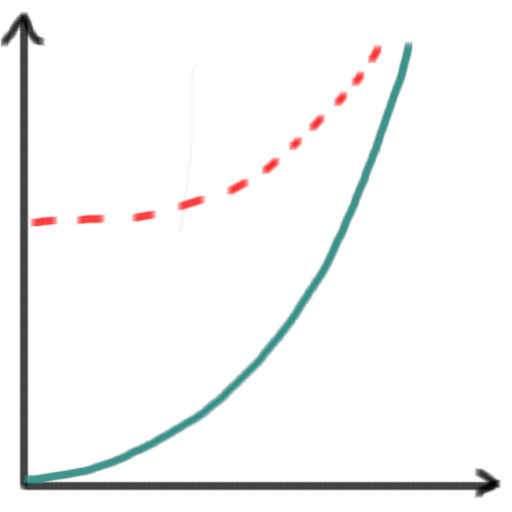
\includegraphics[width=0.5\linewidth]{img/intro/imaginaire-1}
            \caption{Illimité}
        \end{subfigure}
        \begin{subfigure}{.2\textwidth}
            \centering
            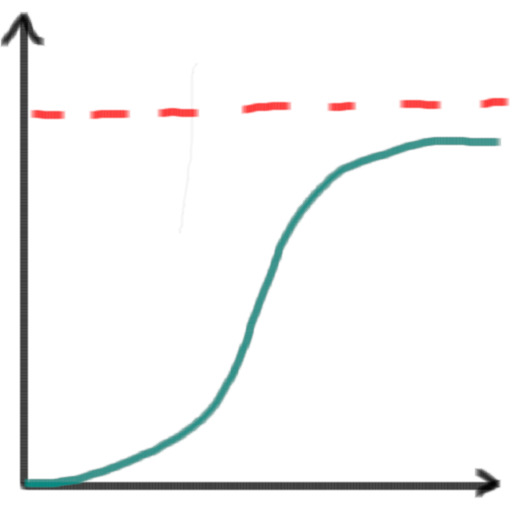
\includegraphics[width=0.5\linewidth]{img/intro/imaginaire-2}
            \caption{Soutenable}
        \end{subfigure}
        \begin{subfigure}{.2\textwidth}
            \centering
            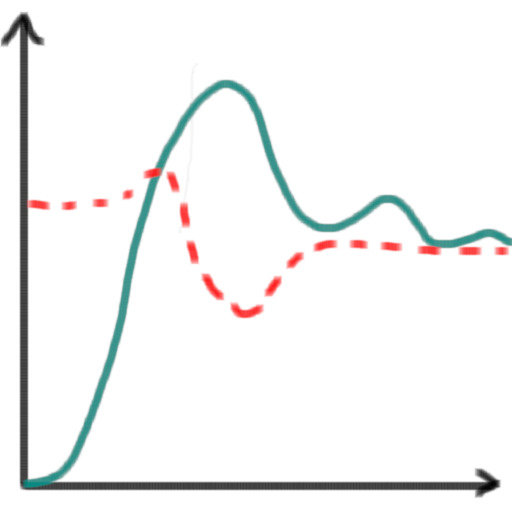
\includegraphics[width=0.5\linewidth]{img/intro/imaginaire-3}
            \caption{Découplage}
        \end{subfigure}
        \begin{subfigure}{.2\textwidth}
            \centering
            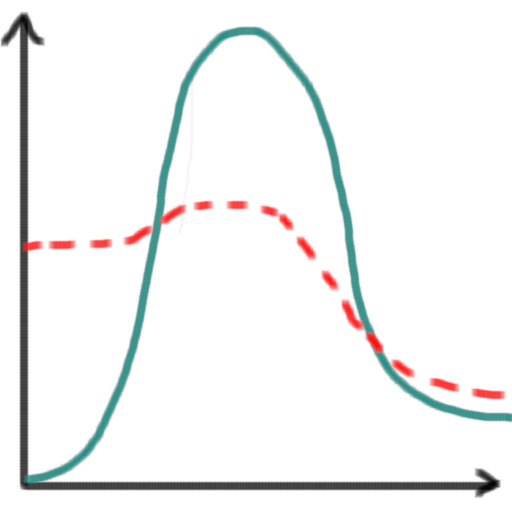
\includegraphics[width=0.5\linewidth]{img/intro/imaginaire-4}
            \caption{Effondrement}
        \end{subfigure}
        \caption{Dynamique des systèmes : les différents imaginaires possibles}
        \label{fig:02-imaginaire}
    \end{figure}
    \vfill
    
    %\vspace{-0.5em}
    \paragraph{Illimité} : % Nous pouvons par exemple montrer que la PAC de 1962 ce situe dans l'imaginaire (a) celui des ``illimitistes'', ou l'on continue de produire toujours plus tout en repoussant sans limite la biocapacité de notre planète.
    Ce scénario est antérieur aux prises de conscience environnementale. La PAC de 1962, orientée vers l'augmentation, d'année en année, des productions agricoles en Europe, s'inscrit dans cette vision.
    
    \vspace{-0.5em}
    \paragraph{Soutenable} : % Depuis peu nous commençons a voir que notre planète à une biocapacité limitée (b) mais que la biocapacité limitée seras capable d'absorber notre empreinte écologique pour tendre vers un univers ``soutenable''. Il en a résulté une modification de la PAC en 1999 avec l'apparition d'exigences environnementales pour rester en dessous de la limite de la biocapacité.
    Postérieur aux prises de conscience environnementales, ce scénario considère une biocapacité limitée, mais suffisante pour absorber l'impact de l'activité humaine. Il en a résulté une modification de la PAC en 1999 avec l'apparition d'exigences environnementales devant permettre de rester en dessous de la limite de la biocapacité.
    
    \vspace{-0.5em}
    %(en cohérence avec le réchauffement climatique et la baisse de la biodiversité)
    \paragraph{Découplage} : Ce scénario, introduit une biocapacité fluctuante, et imagine des dépassements temporaires, avant une convergence progressive entre biocapacité et empreinte. Il s'accompagne d'un découplage de notre croissance économique et de l'empreinte écologique de nos modes de production. Il s'agit d'un modèle de développement durable envisagé par exemple lors des COP (Conference of the Parties), ou de la rédaction du protocole de Kyoto.
    % Ont commence à ce rendre compte que la biocapacité est limité et peut fluctuer (c).
    %L'idée étant de crée un développement durable par exemple avec les COP (Conference of the Parties), le protocol de Kyoto, \dots dont les rapports du GIEC \footnote{Groupe d'experts intergouvernemental sur l'évolution du climat} en sont les conséquences. Tout ce joue donc sur le découplage de notre croissance économie et de l'empreinte écologique de notre mode de production (sans dégât écologique), un défit technique et scientifique difficile.
    
    \vspace{-0.5em}
    \paragraph{Effondrement} : Il s'agit de la perte de la capacité du système à se régénérer. S'ensuit un effondrement de la biodiversité, puis de la production sur une très longue période entraînant une chute démographique brute. Les politiques évoquées précédemment visent à éviter ce scénario. %\footnote{Collapsologie}
    
    %A force de puiser dans nos ressources renouvelables (halieutique, foret, \dots) le système n'arrivera plus à ce régénérer (d). C'est un effondrement de la biodiversité, puis de la production sur une très longue période entrainent une chute démographique brute, c'est une possibilité rarement étudiée \footnote{Collapsologie} et prend un écho particulier avec le réchauffement de la planète. Nous observons par exemple un baise important aux niveaux mondial de la capacité de production des sols, des ressources halieutiques disponible du à leurs sur-exploitation, une chute importante des pollinisateurs du au phytosanitaire et la fonte des glacier d'altitudes qui entrainerons plus fréquemment des sècheresses et des épisodes cévenoles importants \cite{Ph-Martin-2017-et-al-JISTEE-1-2017}.
    
    %\begin{figure}[H]
    %	\centering
    %	%\rotatebox{90}{\scriptsize (source : \href{https://seenthis.net/sites/1501094}{seenthis.net})}
    %	%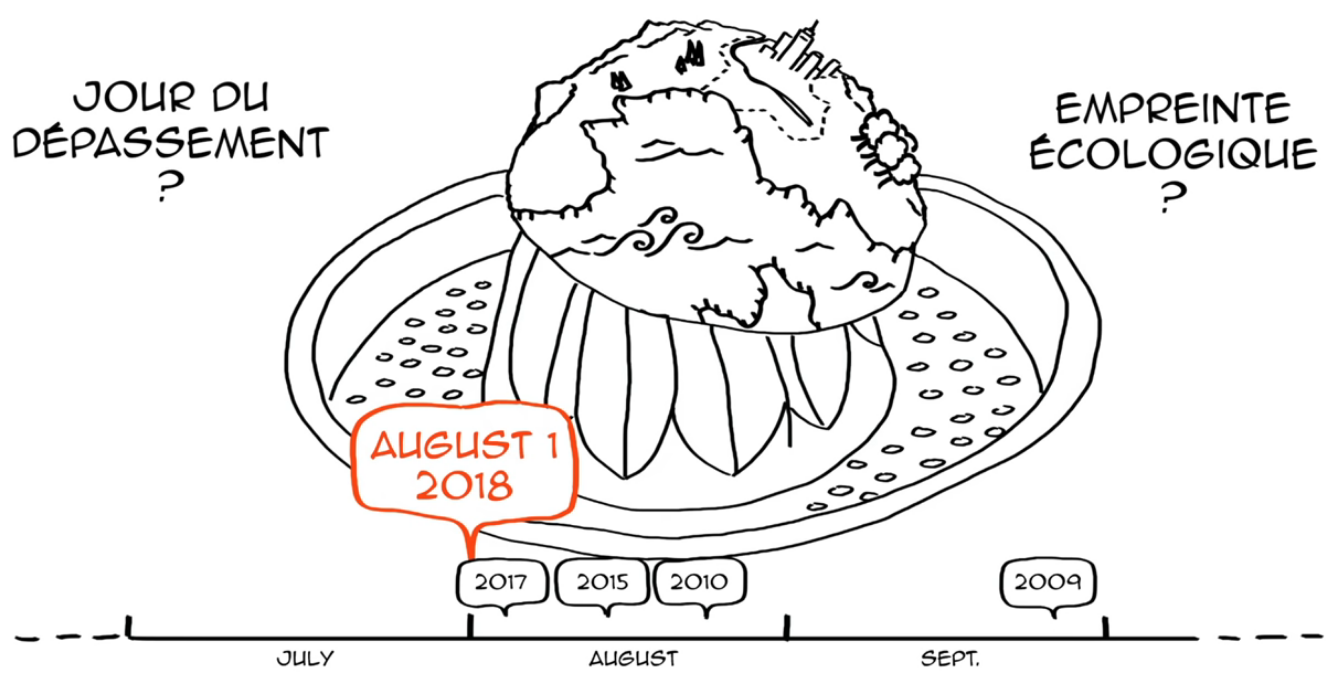
\includegraphics[width=0.6\linewidth]{./img/intro/intro-ressources.jpg}
    %	%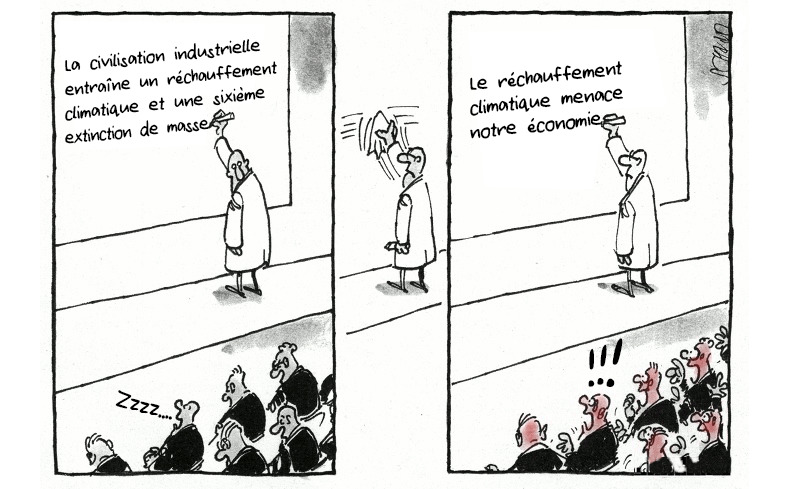
\includegraphics[width=0.7\linewidth]{./img/intro/intro-Climate-change-fr}
    %	\rotatebox{90}{\scriptsize (source : \href{https://www.lemonde.fr/planete/article/2020/01/07/le-recours-aux-pesticides-a-connu-une-hausse-spectaculaire-en-2018_6025101_3244.html}{lemonde.fr})}
    %	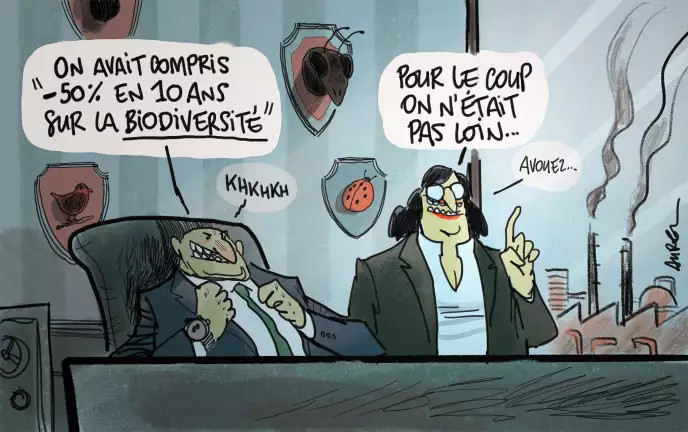
\includegraphics[width=0.5\linewidth]{./img/intro/intro-biodiversiter.jpg}
    %	\caption{Importance de la biodiversité selon les acteurs économiques}
    %\end{figure}
    
    \par Aujourd'hui, nous savons que les deux premiers univers ne sont pas possibles puisque l'on a déjà dépassé la biocapacité de notre planète \cite{meadows1972limits, day2017earth}. Et nous observons une baisse significative, aux niveaux mondiaux, de la capacité de production des sols, des ressources halieutiques, du nombre de pollinisateurs et la fonte des glacier d'altitudes \cite{perrier2013anthropocene, Ph-Martin-2017-et-al-JISTEE-1-2017}. Il est donc urgent aujourd'hui de reconsidérer nos modes de production. Et plus largement les bases de notre économie qui représente un défi scientifique et technologique majeur \cite{carles2007volem, aberkane2015economie, jancovici2017avenir}. %Ces questions n'ont pas encore de réel réponse politiques \cite{doi:10.1080/09640560123782}.
    
    \newpage
    \subsection{Limites de l'agriculture intensive}
    \label{sec:02-limit-of-intensive-agriculture}
    \subsubsection{Impact de la mécanisation}
    
    L'intensification de l'agriculture française se développe à partir de 1950 en France à travers le plan Marshall. La mécanisation permet la réduction de la pénibilité du travail physique, l'automatisation de certaines tâches quotidiennes et des débits de chantier élevés, permettant un gain de productivité notable. Le gouvernement français, soutenu par la PAC, lance alors le remembrement des terres agricoles peu avant 1970, pour faciliter l'usage des matériels agricoles et la simplification des interventions culturales. On estime ainsi que \SI{40}{\percent} a \SI{80}{\percent} des bocages ont disparu (figure \ref{fig:02-intro-bocage}), et le remembrement des terres agricoles continue au fil des générations.
    
    %Les premiers tracteurs fond leurs apparition en 1950 en France à travers le plan Marshall, permettant la mécanisation de l'agriculture. Cette modernisation de l'agriculture française, est tout d'abord apparue comme bénéfique par l'agriculteur avec la réduction de la pénibilité du travail physique, l'automatisation de certaines tâches quotidiennes et des débits de chantier élevés de ces machines puissantes, permettant un gain de temps notable. Le gouvernement français, soutenue par la PAC, lance alors le grand remembrement des terres agricoles peu avant 1970, pour faciliter leurs usages. On estime ainsi que \SI{40}{\percent} a \SI{80}{\percent} des bocages ont disparues (figure \ref{fig:02-intro-bocage}), et le remembrements des terres agricoles continue au fils des générations. %Mais nous allons voir que les conséquences ne sont pas anodines.
    
    \vfill
    \begin{figure}[H]
        \centering
        %\rotatebox{90}{\scriptsize (source : \href{https://www.tela-botanica.org/2019/02/le-bocage-un-milieu-qui-ne-haie-pas-la-biodiversite/}{tela-botanica.org}) } 
        \source{\cite{boissinot2014terres}}
        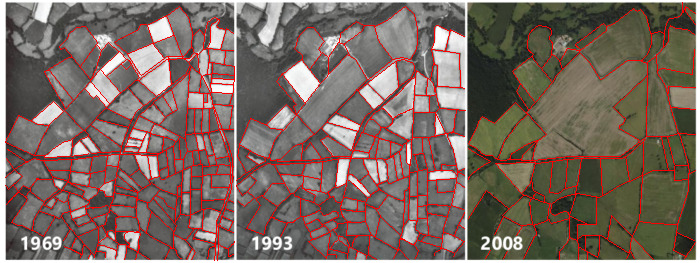
\includegraphics[width=0.6\linewidth]{img/intro/intro-bocage-2}
        \caption{Remembrement des terres agricoles}
        \label{fig:02-intro-bocage}
    \end{figure}
    \vfill
    
    %\begin{wrapfigure}{r}{4.0cm}
    %	\centering
    %	\vspace{-1.em}
    %	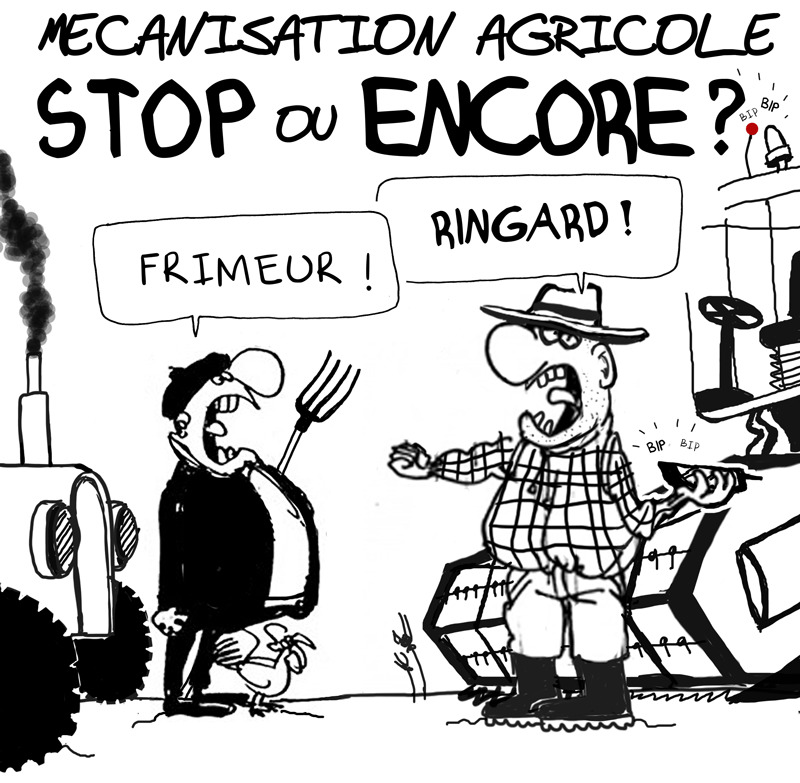
\includegraphics[width=3.3cm]{img/intro/intro-mechanisation}
    %	\rotatebox{90}{\scriptsize (source : comicearlon.be)}
    %	\label{fig:02-intro-mechanisation}
    %	\vspace{-1.em}
    %\end{wrapfigure}
    
    % https://ree.developpement-durable.gouv.fr/themes/milieux-et-territoires-a-enjeux/sols-et-sous-sol/fertilite-et-biodiversite/article/la-biodiversite-des-sols
    Avec l'apparition de grandes terres agricoles, les besoins en équipements agricoles évoluent et des progrès techniques considérables y font leurs apparitions afin d'être de plus en plus compétitifs sur les marchés. L'intensification de nouvelles pratiques (labour profond, engrais chimiques) entraînent lentement une disparition de la matière organique des sols \cite{vitinnov2017journees} qui sert d'alimentation à la faune et flore des sols \cite{pujol2014journee} tel que les lombrics \cite{pelosi2008modelisation}, les carabes \cite{carbonne:tel-03163078} et les mycorhizes \cite{zerbib2018relations}.
    % lombric \footnote{\url{https://ree.developpement-durable.gouv.fr/}}
    
    \par Ces pratiques intensives, mettent également les sols à nu, impliquant un phénomène de tassement et compactage des sols. Ce dernier freine le développement des racines et la pénétration de l'eau dans les couches inférieures, utiles aux cultures, par exemple comme réserve d'eau en cas de sécheresse ou le stockage de certains éléments comme l'azote et le carbone \cite{dos2009crop, nemery2016carbon, kan2020responses}. Puisque l'eau ne pénètre plus, elle ruisselle en surface et \og entraîne une acidification des sols par perte du calcium, lequel sert de pont d'attache entre les argiles et les humus. Sans calcium, le complexe argilo-humique se détruit et les argiles partent en suspension dans l'eau. Enfin, il y a l'érosion \fg     
    %\rlap{\textcolor{white}{\hypersetup{citecolor=white}\cite{bourguignon2008sol}}}
    {\cite{ANTHONY2012268, YOUSEFI201655, cossart2019erosion, hinimbio:tel-02305183, kolli2021estimation}.}
    
    
    \par Ces deux facteurs menacent ainsi la durabilité de la production par une pollution environnementale (eau, sol, air), un appauvrissement des sols et une réduction de la biodiversité. Aujourd'hui un regain d'intérêt pour les bocages se fait ressentir, ainsi de nombreuses études ont montré qu'à l'échelle du paysage, les habitats peu perturbés comme les haies ou les prairies jouent un rôle important pour le maintien et le déplacement de certains auxiliaires, mais également dans la gestion et le ralentissement du lessivage des sols. À contrario, les petites parcelles qui n'ont pu être remembrées sont abandonnées dû à plusieurs facteurs, comme la pénibilité du travail. Les parcelles abandonnées s'enfrichent \cite{pic:hal-03008309} faisant temporairement office de réserve à la bio-diversité. Après un certain temps, les friches tendent soit vers la forêt, soit à la reprise, soit vers l'urbanisation en fonction des acteurs économiques à proximité.
    
    % carbon <-> mycor\cite{soudzilovskaia2019global}
    % Une complémentarité des ressources entre les cultures et les haies adjacentes l'échelle du paysage est dominés par des parcelles gérées extensivement.
    
    %\begin{figure}[H]
    %	\centering
    %	\rotatebox{90}{\scriptsize (source : \href{http://www.donnees.statistiques.developpement-durable.gouv.fr/lesessentiels/essentiels/sol-perte-compactage.html}{statistiques.developpement-durable.gouv.fr})}{}
    %	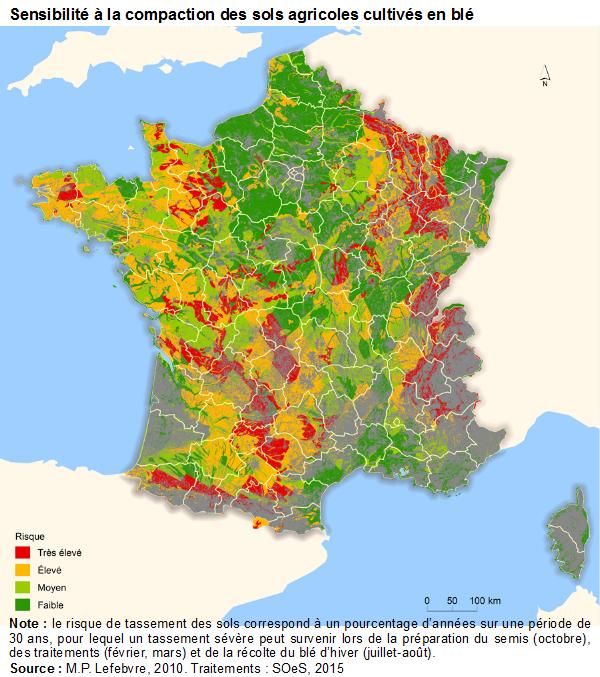
\includegraphics[width=0.3\linewidth]{img/intro/compaction}
    %	\caption{}
    %	\label{fig:02-compaction}
    %\end{figure}
    
    %\newpage
    %\subsection{Diversité génétique}
    %
    %	Avec l'augmentation de la taille des parcelles, c'est toute une diversité génétique qui s'effrite au fils des années. C'est aussi l'arriver des semenciers, les agriculteurs achètes leurs graines, au lieu de les produire et ressemer, d'ailleurs cette pratique fut ``interdite'' a partir du 18 mai 1981 avec l'apparition d'un catalogue Européen des semences, celles non-inscrites ne peuvent des l'hors plus être commercialisés. C'est donc le début de l'homogénéisation des variétés et l'abandon progressif des semences paysannes et traditionnelles. Pour le blé c'est plus de 2700 variétés qui était cultivées en France (conserver a l'INRA), dont une vingtaine sont encore cultivées.
    %	\\
    %	%\par Il existais quelques 6 000 variétés de pommiers et poirier, pourtant seulement 12 de pomme et 6 de poire y sont inscrite.
    %	% http://www.pommiers.com/pomme/pommier.htm
    %	% https://www.aujardin.info/fiches/pommes-commerciales-dites-modernes.php
    %	%Chaque variété était adaptés a sont climat, a sont utilisation aussi parfois : La coeur de piegon, la bergamotte de balege, la poire suce lait, la poire sans regle, la culotte suissse, la poire etoufe chrétien, la pomme museaux de veaux, la pomme de glace, la poire cuisse dame, la poire trompe laron, la cuillard etrangleuse \dots Pour le blé c'est plus de 2700 variétés qui était cultivées en France (conserver a l'INRA), dont une vingtaine sont cultivées.
    %	
    %	\par L'industrie agroalimentaire a sélectionné les variétés les plus ``belles'' et les plus productives, mais rarement les plus riches sur le plan nutritif et apporte donc son lot d'avantages et d'inconvénients. Prenons pour exemple le cas des blés meuniers qui via la sélection génétique et l'hybridation (polyploïdisation), est passé de 14 a 42 chromosomes aux fils des adaptation. Ce qui a augmenté leurs rendements par 3-4 entre 1990 et 2018 \cite{Geneviève2018}. Cela à également permis l'obtention de teneurs en gluten plus importantes et des chaînes amidonnées plus longues, permettant d'augmenter la vitesse de pétrissage pour la fabrication du pain, mais les rendent difficile à assimiler par l'organisme humain. Ainsi des problèmes de santé publique sont apparus (intolérance au gluten). D'autres exemples sont intéressant, on observe une forte diminution de la quantité de vitamine dans les pommes (\SI{90}{\percent}) et dans les carottes (\SI{75}{\percent}) entre 1947 et 1990 en France. De nombreuses études sur le sujet rapporte des résultats similaires à travers le globe \cite{christian2002charts, USDA_Food, halweil2007still}. Ces études doivent néanmoins être prises avec précautions, car ces effets sont également provoqués par d'autres facteurs tel-que des récoltes trop précoces ou des cultures sous-serre hors saisons. 
    %	
    %	\begin{figure}[H]
    %		\centering
    %		\rotatebox{90}{\scriptsize (source : \href{http://www.bourgogne-nature.fr/fichiers/revues/pages_026a039_de_bfcn27_cahiers_ld.pdf}{bourgogne-nature.fr}) }
    %		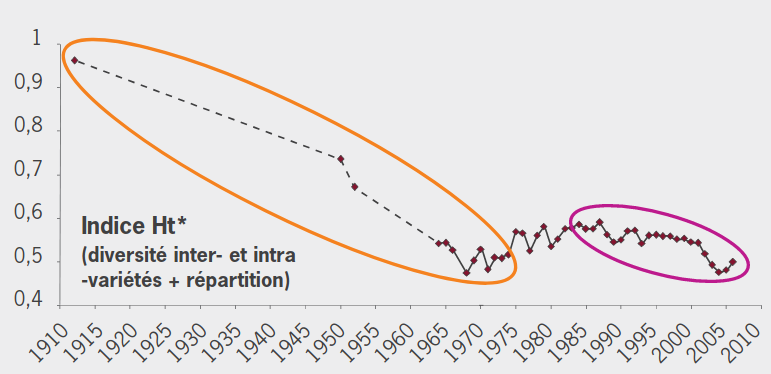
\includegraphics[width=0.5\linewidth]{img/intro/variete-genetique-ble}
    %		\caption{Diversité génétique du blé tendre en France depuis un siècle}
    %		\label{fig:02-variete-genetique-ble}
    %	\end{figure}
    %
    %	% https://www.nouvelobs.com/rue89/rue89-planete/20150126.RUE7557/une-pomme-de-1950-equivaut-a-100-pommes-d-aujourd-hui.html
    %	% https://www.lexpress.fr/styles/saveurs/pourquoi-les-bles-anciens-vont-changer-votre-pain-quotidien_2034554.html
    %	% https://www.pourlascience.fr/sr/chroniques-de-levolution/comment-le-ble-est-devenu-tendre-15158.php
    %	% C'est donc un retour progressif vers d'anciennes variétés qui ce manifeste.
    %	
    %	\par L'érosion de la diversité génétique des cultures, couplés a de grandes parcelles (sans bocages) a aussi favorise la propagation et l'adaptation de maladie. Ressemant, le ``xylella fastidiosa'', appelé ``la lèpre des oliviers'', a causé la mort d'un million d'arbres en Italie entre 2013 et 2019.
    %	Plus ancien, c'est le phylloxéra qui a fait des ravages en France sur les vignes entre 1863 et 1869.
    %	Pour le blé c'est différents types de champignon tel-que ``Tilletia caries'', les ``Septoriose'', les ``Fusariose'', les ``Charbon nu'' ou encore ``Claviceps purpurea'' qui fait des ravages. Aujourd'hui le seule moyen de lutte sont les anti-fongiques dont 2 a 4 applications sont couramment effectuées par récoltes.
    %	Pourtant d'autres moyens de contrôle serait possible, tel-que les associations de cultures et certaines adventices pressentant des services écosystémiques. Tout cela permet de dire qu'il existe différent levier sur la réduction de l'utilisation des produits de synthèse, un axe diversité génétique et un axe ``high tech'' via l'agriculture de précision et les OGM.
    %	
    %	\colorbox{orange}{delete page ?}
    
    \subsubsection{Impact des intrants}
    \label{sec:impact-surprod}
    
    Parallèlement au développement de la mécanisation, l'usage de la fertilisation chimique et des traitements phytopharmaceutiques se développe massivement, permettant d'augmenter des rendements et d'alimenter le marché mondial. Leurs utilisations deviennent nécessaires puisque les sols s'appauvrissent avec l'intensification. Lors de fortes pluies et du fait de la suppression des bocages, les polluants sont lessivés puis ruissellent vers les rivières \cite{tournebize2020, pic2022mais}. C'est le cas des fertilisants, visible sur la figure \ref{fig:02-intro-carte-azote} pour les excédents d'azote.
    
    
    %\begin{wrapfigure}{r}{4.0cm}
    %	\centering
    %	\vspace{-1.em}
    %	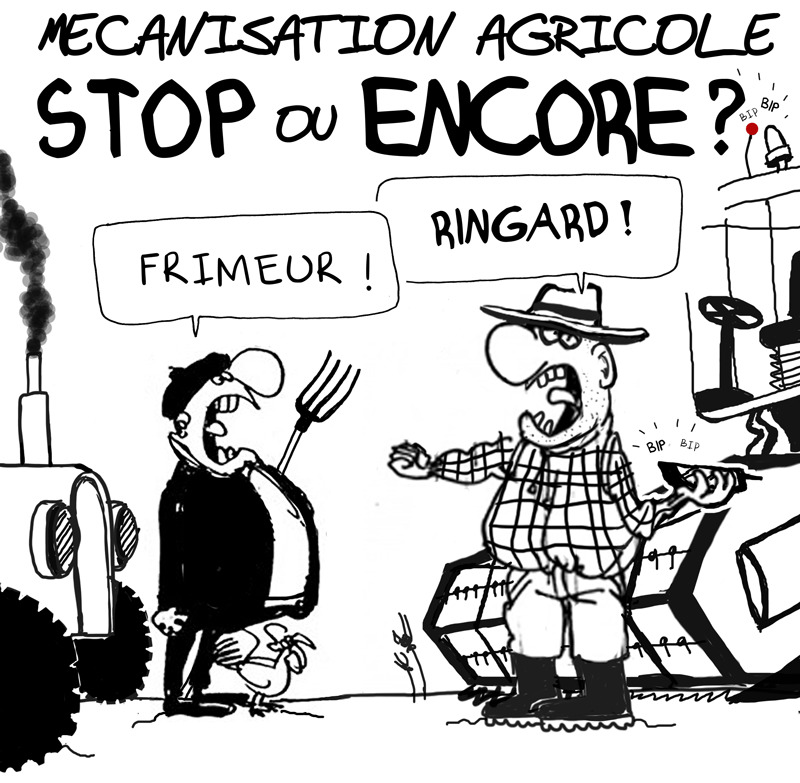
\includegraphics[width=3.3cm]{img/intro/intro-mechanisation}
    %	\rotatebox{90}{\scriptsize (source : comicearlon.be)}
    %	\label{fig:02-intro-mechanisation}
    %	\vspace{-1.em}
    %\end{wrapfigure}
    
    %\begin{wrapfigure}{r}{7.5cm}
    %%\begin{figure}[H]
    %	\centering
    %	%\rotatebox{90}{\scriptsize (source : \href{https://www.charles-de-flahaut.fr/scolaire/evolution_campagnes.htm}{charles-de-flahaut.fr}) }
    %	%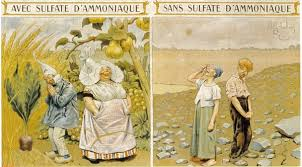
\includegraphics[height=4.0cm]{img/intro/intro-engrais}
    %	%\hfill
    %	{\scriptsize (source : wikipedia.fr) }
    %	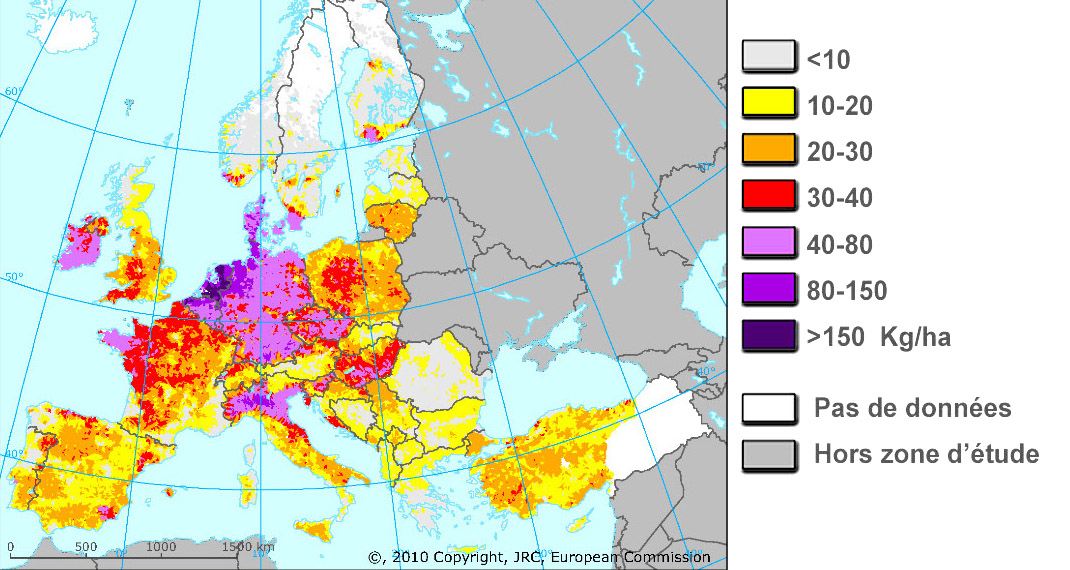
\includegraphics[height=4.0cm]{img/intro/intro-carte-azote}
    %	\caption{Excédent d'azote en 005}
    %	\label{fig:02-intro-carte-azote}
    %%\end{figure}
    %\end{wrapfigure}
    
    \vfill
    \begin{figure}[H]
        \centering
        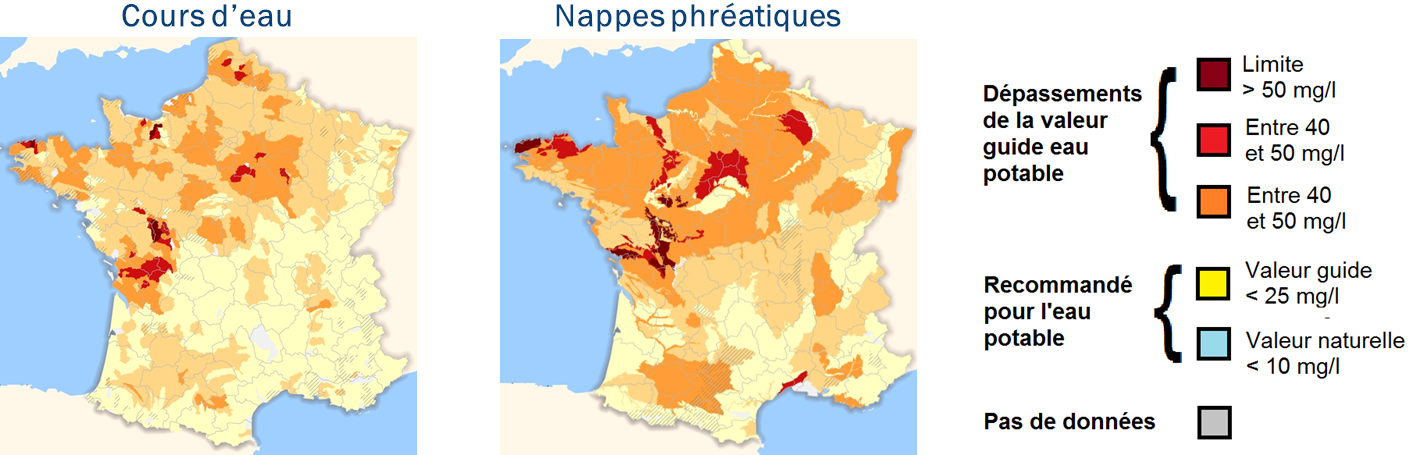
\includegraphics[width=\linewidth]{img/intro/intro-carte-azote-2}
        {\scriptsize (source : Agences et offices de l'eau / SOeS, 2016) }
        %{\scriptsize (source : wikipedia.fr) } \\
        %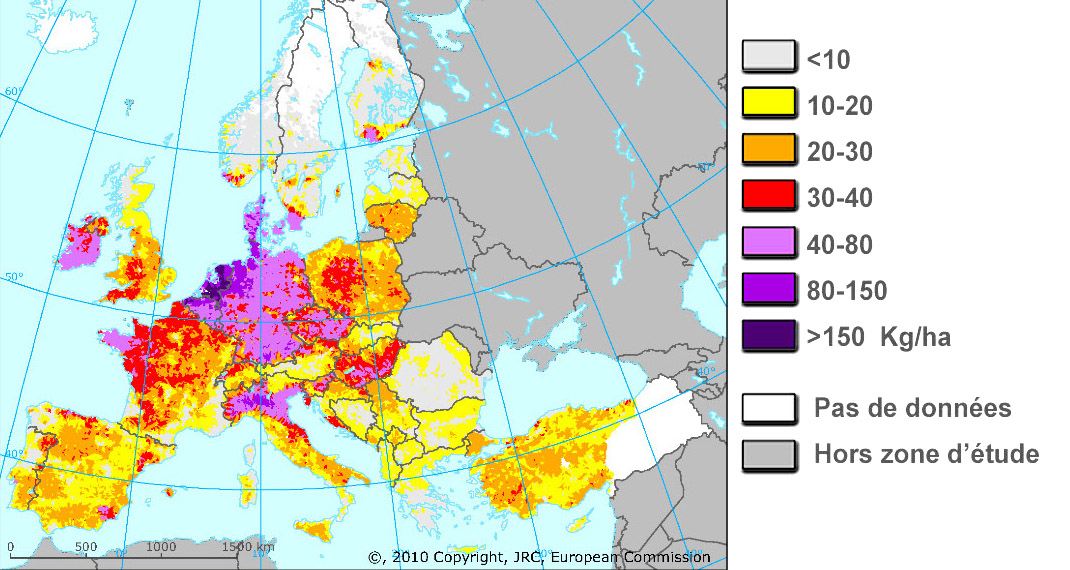
\includegraphics[width=0.7\linewidth]{img/intro/intro-carte-azote}
        \caption{Excédent d'azote dans la majorités des cours d'eau en 2013}
        \label{fig:02-intro-carte-azote}
    \end{figure}
    \vfill
    
    \par L'excès de nutriments dans les rivières induit une prolifération d'algues et de cyanobactéries qui se développent en masse et entraînent à terme la limitation de la pénétration de la lumière dans la colonne d'eau (en particulier dans les barrages). Ensuite, les algues légèrement sous la surface meurent et tombent au fond entraînant une dégradation de matière organique consommant l'oxygène du milieu (désoxygénation), puis à terme l'asphyxie du milieu aquatique (mort des poissons). C'est l'eutrophisation des milieux aquatiques ! 
    
    \par L'eutrophisation d'origine anthropique est donc due à l'intensification des modes de productions et l'usage de fortes doses. Le phénomène des algues vertes \cite{léraud2019algues}, comme les Sargasses dans les Caraïbes \cite{louime2017sargassum} sont alimentées par \SI{95}{\percent} des nutriments azotés provenant de la lixiviation des terres agricoles et donc des fertilisants agricoles. De plus, dans le golfe du Mexique une immense « zone morte » grandit le long de la Louisiane et du Texas (estimée à 22 000 kilomètres carrés) provoquée par l'asphyxie, ici du Mississippi. Ces trois exemples importants sont visibles en figure \ref{fig:02-intro-limites-algues}.
    
    %\newpage \null
    \vfill
    \begin{figure}[H]
        \centering
        {\scriptsize (source : www.ouest-france.fr) } \\
        
        \begin{subfigure}{.3\textwidth}
            \centering
            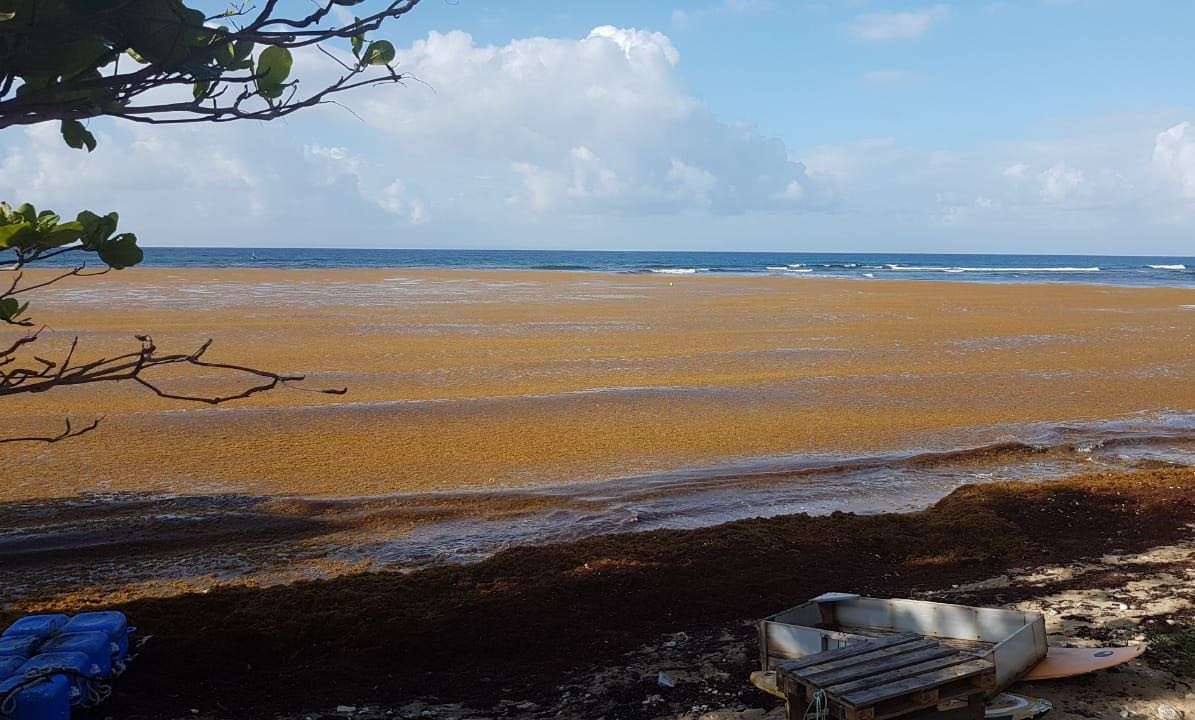
\includegraphics[width=\linewidth]{img/intro/intro-limites-sargas} \\
            \scriptsize Guadeloupe
        \end{subfigure}
        \hfill
        \begin{subfigure}{.3\textwidth}
            \centering
            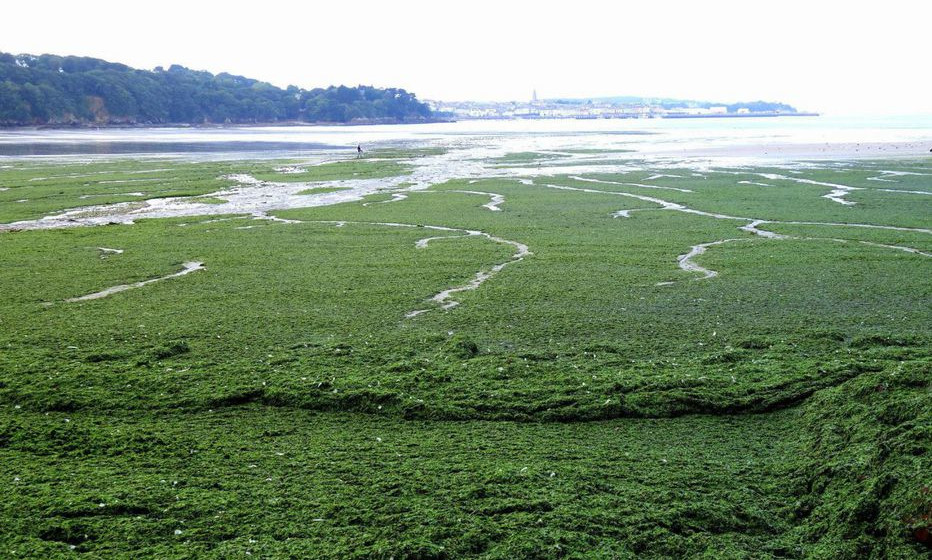
\includegraphics[width=\linewidth]{img/intro/intro-limites-algues-vertes} \\
            \scriptsize Bretagne
        \end{subfigure}
        \hfill
        \begin{subfigure}{.3\textwidth}
            \centering
            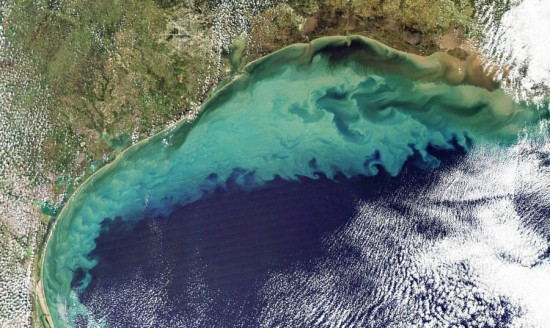
\includegraphics[width=\linewidth]{img/intro/intro-limites-zone-norte} \\
            \scriptsize Golfe du Mexique
        \end{subfigure}
        \caption{Prolifération d'algues et asphyxie des milieux aquatiques}
        \label{fig:02-intro-limites-algues}
    \end{figure}
    \vfill
    
    \newpage
    Ces algues ont également des conséquences importantes sur la santé humaine. Les gaz émis par leur décomposition sont hautement toxiques (hydrogène sulfuré et ammoniac) dont leur inhalation peut entraîner la mort, plusieurs cas ont été reportés depuis 1984 en Bretagne. La loi sur \href{https://fr.wikipedia.org/wiki/Loi\_sur\_l\%27eau_et_les_milieux_aquatiques}{l'eau et les milieux aquatiques du 30 décembre 2006} (LEMA) tente de limiter ces effets.
    
    \par Comme nous l'avons vu pour les fertilisants, les pesticides sont également emportés par le lessivage des terres agricoles \cite{tournebize2020}. Un rapport du ministère de la Transition écologique et solidaire de juin 2017 fait état des pesticides présents sur presque tout le territoire français, mais à des concentrations variables (figure \ref{fig:02-intro-carte-pesticide}).
    
    \begin{figure}[H]
        \centering
        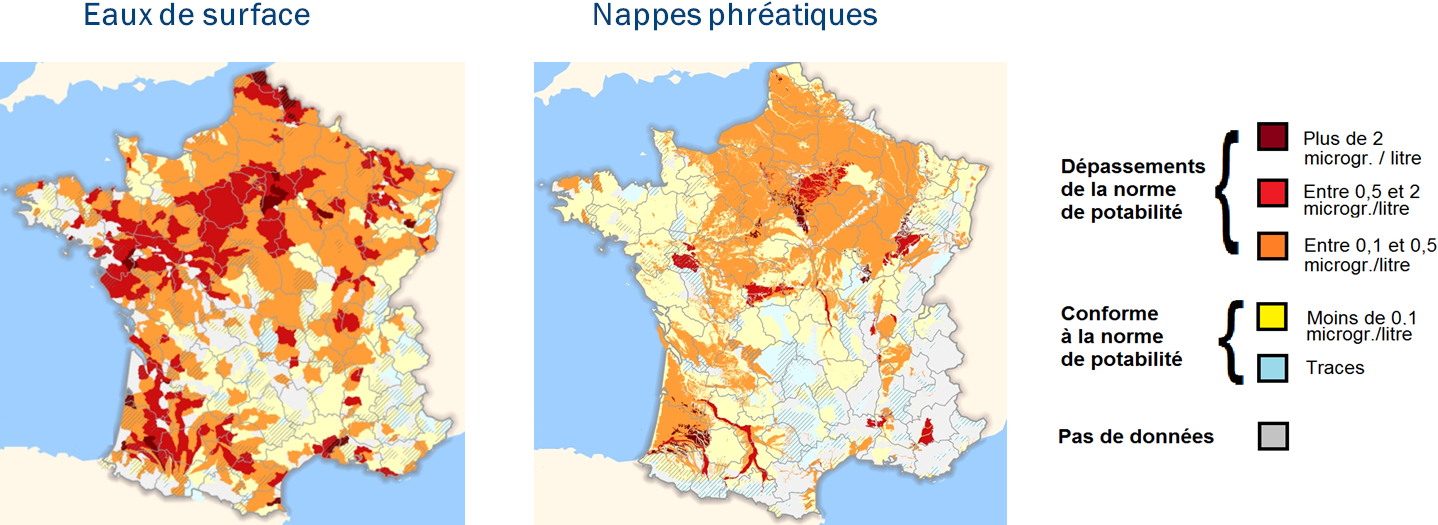
\includegraphics[width=\linewidth]{img/intro/intro-carte-pesticide-2}
        {\scriptsize (source : Agences et offices de l'eau / SOeS, 2016) }
        % http://www.ipreunion.com/volcan/reportage/2018/03/28/un-rapport-accablant-des-pesticides-dans-la-quasi-totalite-des-eaux-reunionnaises,79264.html
        %{\scriptsize (source : wikipedia.fr) }
        %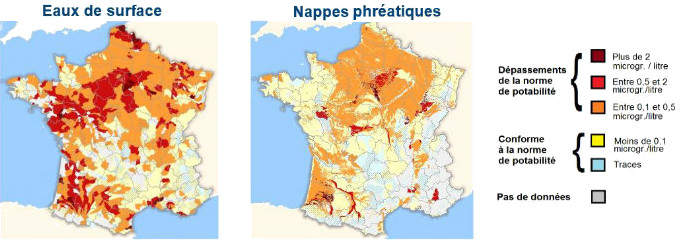
\includegraphics[width=\linewidth]{img/intro/intro-carte-pesticide}
        \caption{Presence de pesticide dans la majorités des cours d'eau en 2013}
        \label{fig:02-intro-carte-pesticide}
    \end{figure}

    Plusieurs publications ont mis en évidence les effets néfastes des pesticides sur l'environnement \cite{MCLAUGHLIN1995201, vanderwerf1997, Pesce2021} impliquant une dégradation des écosystèmes \cite{aubertot2005pesticides, bianchi2006sustainable}. D'après \cite{GEIGER201097}, sur les 13 composantes de l'intensification agricole qui ont été mesurées, l'utilisation d'insecticides et de fongicides a eu des effets négatifs constants sur la biodiversité. Il est important de noter que les pesticides sont généralement appliqués par pulvérisation, impliquant une forte volatilisation du produit, qui peut s'échelonner de quelques jours à plusieurs semaines. Engendrant un transfert de masse dans l'atmosphère \cite{bedos2002mass} et touchant donc des populations non-ciblées. Ceci implique des effets collatéraux, importants, sur la diversité des espèces de plantes sauvages, de carabes et d'oiseaux \cite{GEIGER201097}, et donc sur le potentiel de lutte biologique contre les ravageurs. Les populations d'invertébrés sont également touchées \cite{Mikhail2013, grozinger2019bee, wood2020managed}. 
    
    Concernant les espèces humaines et animales, l'exemple de l'utilisation du Chlordécone, pesticide utilisé dans les Antilles Françaises, pour traiter les plants de bananes, a montré un impact négatif \cite{DUBUISSON20075, maudouit2019systematic}. Les conséquences possibles à long terme continuent d'être étudiées, car le Chlordécone contamine encore les sols des Caraïbes. Les effets d'une exposition aiguë sont bien décrits, en revanche les effets à des doses plus diffuses se précisent, même s'ils restent complexes à identifier.
    
    Face à ces éléments (engrais, pesticides, pratiques intensives, \dots), \og il est clair que nous devons trouver des solutions techniques afin de maximiser l'intégrité de l'écosystème et le bien-être de l'homme sans affecter notre avenir \fg \cite{dufour2009myth}.
    %, ce qui favorise la conservation des valeurs écologiques ainsi que leur fonction sociologique et économique de façon durable
    
    %La présence de ces pesticides arrive également jusqu'à nos assiettes et \SI{100}{\percent} des urines des Français contiennent également des traces de glyphosate. Parallèlement, on observe une chute drastique du nombre de spermatozoïdes chez les hommes et une forte augmentation des tumeurs du sein chez les femmes \cite{SurveillanceAlimentaires, bircher1943hounza}. Ces phénomènes sont considérés comme liés notamment par les pesticides, dont les composés organochlorés sont considérés comme responsables probables par l'OMS et l'Anses \cite{myers2016concerns, de2021cancer}.
    
    %Le travail effectué dans cette thèse s'intéresse spécifiquement à une gestion localisée des adventices dans le cadre d'une transition agroécologique et approche d'agriculture de précision. La section \ref{sec:place-adventice} suivante détaille la place des adventices dans les systèmes de culture et leur mode de gestion.
    
    
    
    \newpage
    \subsection{Modes de production}
    
    %Actuellement, l'agriculture conventionnelle et l'agriculture biologique sont les modes de production les mieux connus. Face à la volonté de préserver l'environnement et l'évolution des pratiques, d'autres types d'agricultures, dites ``alternatives'' se sont mises en place : l'agriculture durable, l'agriculture de précision, l'agriculture de conservation, l'agriculture raisonnée, l'agriculture intégrée, l'agriculture multifonctionnelle, la permaculture, l'hydroponie \dots dont les principes sont développés ci-dessous pour contextualiser notre domaine d'application. De plus, pour chaque mode de production, quelques articles sont également mis en exergue montrant certaines limites et/ou des changements sociétaux nécessaires.
    
    %! JNP
    Actuellement, l'agriculture dite ``conventionnelle'' constitue le mode de production de référence des sociétés industrielles. Elle a recours à divers intrants chimiques de synthèse \cite{kisinyo2011epuisement} pour maintenir l'état sanitaire de la culture face aux différents stress biotiques \cite{pandey2017impact} et abiotiques \cite{cramer2011effects} qu'elle peut subir. Face aux préoccupations environnementales, mais également pour répondre aux attentes des consommateurs (en termes de risque sanitaire \cite{SurveillanceAlimentaires} et de qualité nutritive des aliments), différentes évolutions ont été envisagées pour l'agriculture conventionnelle, et des modes de production alternatifs ont été définis, dont les principaux sont :
    
    %\paragraph{Agriculture conventionnelle} :
    %Ce type d'agriculture a recours aux produits chimiques de synthèse pour maintenir l'état sanitaire de la culture face aux différents stress qu'elle peut subir : stress abiotiques (sécheresse, changement climatique, ressources, lumière, \dots \cite{cramer2011effects}) ou stress biotiques (bioagresseurs : ravaveurs, adeventices, pathogènes, \dots \cite{pandey2017impact}) qui engendre par exemple des maladies \cite{caquet2020agroecologie}. A terme, cette agriculture est nocive pour la santé des êtres vivants. Le tassement des sols par les engins agricoles, l'érosion des sols par les pluies, la contamination de ceux-ci par les pesticides, fongicide, insecticide, et métaux lourds contribuent à la destruction de la vie dans les sols \cite{bourguignon2008sol}. Les sols ne fabriquent plus leurs propres matières organiques, renforçant ainsi l'emploi d'engrais à forte dose. Les terres arables sont réduit à leurs plus simples rôles de sols inertes.
    
    %\vspace{-0.5em}
    %\begin{itemize}
    %	\item Phosphate le plus gros gisement au monde en fin de resserve ? \cite{kisinyo2011epuisement}
    %	%\item Pétrole une ressource limitée (pétrochimie, intrant, pesticide, carburant) \cite{}
    %	\item Résidus de pesticides dans l'alimentation et risques sanitaires \cite{SurveillanceAlimentaires}
    %\end{itemize}
    %\vspace{-1em}
    
    \paragraph{Agriculture durable} :
    Dérivée de l'agriculture conventionnelle, c'est une agriculture extensive qui s'inscrit dans les perspectives ouvertes par le développement durable défini en 1992 à Rio \footnote{\url{https://fr.wikipedia.org/wiki/Agenda_21}}. Ce type d'agriculture vise à \og répondre aux besoins du présent sans compromettre la capacité des générations futures à répondre à leurs propres besoins \fg. Il s'agit donc de moduler nos productions pour concilier les dimensions écologiques, économiques et sociales. Ce concept n'est pas appuyé par une législation précise.
    
    %\paragraph{Hydroponie} :
    %Dernièrement, un mode de culture hors-sol fait également sont apparition dans les villes pour coloniser les surfaces verticales.
    %Ce mode de production ce réalise sur un substrat neutre et inerte (sable, billes d'argile, laine de roche, plastique, \dots),
    %il est régulièrement irrigué d'un courant de solution qui apporte des sels minéraux et des nutriments essentiels à la plante.
    %Mais des pesticides ou produits sanitaires sont souvent utilisés dans ce type de production.
    %
    %\begin{itemize}
    %	\item En depit de l'usage d'intrant, l'hydroponie pourrait être une solution a la pollution
    %	et l'augmentation des températures dans les villes \cite{montiel2015proPgramme} (mur et toit végétalisé)
    %\end{itemize}
    
    \paragraph{Agriculture biologique} : Il s'agit du mode de production alternatif le plus connu. Son objectif est d'intégrer un ensemble de pratiques agricoles plus respectueuses des équilibres écologiques, du bien-être des animaux et de l'autonomie des agriculteurs. Cette agriculture a pour particularité d'exclure l'usage des produits chimiques de synthèse \cite{WINTERMANTEL2020135400}, des OGM \cite{Bagnoud2020} et limite l'emploi d'intrants \cite{etter2011low}. Les produits issus de ce mode de production font l'objet d'une certification (variable en fonction de l'origine du produit).
    
    %\begin{itemize}
    %	\item Le Sikkim en Inde est le premier état à être \SI{100}{\percent} bio. \cite{Bagnoud2020}
    %	\item Le Siddhipur au Népal travail sur des alternatives au Phosphate. \cite{etter2011low}
    %	\item Cuba est également un bonne exemple, ou l'embargos américain empêchant l'importation de produit phytosanitaire dont les Néonicotinoïdes \cite{WINTERMANTEL2020135400} ont préserver leurs pollinisateurs faisant d'eux le premier exportateur mondial de miel.
    %	\item L'agriculture biologique fait de plus l'objet d'une règlementation ferme en Europe, mais le libre échange la rend également caduque sur certain aspects. C'est le cas de la banane, l'utilisation de pesticide y étant exclue en Europe, mais autoriser en Dominique, l'importation des bananes dominiquaise est tout de même considérer ``BIO'' en Europe.
    %\end{itemize}
    
    \paragraph{Permaculture} : La permaculture est un ensemble de principes de conception centrés sur une pensée systémique globale au sein d'une petite surface. Ce mode de production se rapproche de l'agriculture biologique, mais conçoit son système autour de l'agriculteur, de la famille et de l'habitat. L'exploitation est alors divisée en plusieurs zones fournissant des services différents (jardin annuel, jardin permanent, verger, fourrages, forêt). La permaculture prend également écho dans le domaine des semences libres et paysannes \cite{shiva2005globalization, mesini2006preservation, zerbib2018relations, ElAmine2018}. En Autriche, le Krameterhof  \cite{holzer2011sepp}, la ferme du Bec Hellouin en France \cite{mesini2006preservation} et Fukuoka au Japon \cite{fukuoka1983revolution} sont les exemples les plus connus.
    
    %La permaculture est un ensemble de principes de conception centrés sur la pensée systémique globale au sein d'une petite surface. Ce mode de production ce rapproche de l'agriculture biologique, mais conçoit sont système autour de l'agriculteur, de la famille et de l'habitat. L'exploitation est alors divisé en plusieurs zones proposant des services économiques, écologiques et permanente en fonction de la distance à l'habitat. Ont distingue par exemple le jardin annuel, le jardin permanent, les vergés, les fourrages, et la foret. Mais plusieurs concepts existent, c'est probablement le type d'agriculture le plus en vogue dans les zones rurales. La permaculture prend également écho dans le domaine des semences libres/paysannes.
    
    %\begin{itemize}
    %	\item Inde : biodiversités et les semences libres \cite{shiva2005globalization}
    %	\item Brésil et Venezuela : Résistance massive pour les semences paysannes \cite{mesini2006preservation}
    %	\item Autriche, le Krameterhof : la ferme en permaculture de Sepp Holzer \cite{holzer2011sepp}
    %	\item France, ferme du Bec Hellouin : la beauté rend productif \cite{morel2016ferme}
    %	\item France, Potager de santé : Pascal Poot \cite{zerbib2018relations, ElAmine2018}
    %\end{itemize}
    
    %\begin{figure}[H]
    %	\centering
    %	\source{\href{https://transitionnetwork.org/news-and-blog/commencer-petit-lhistoire-du-bec-hellouin/}{transitionnetwork.org}}
    %	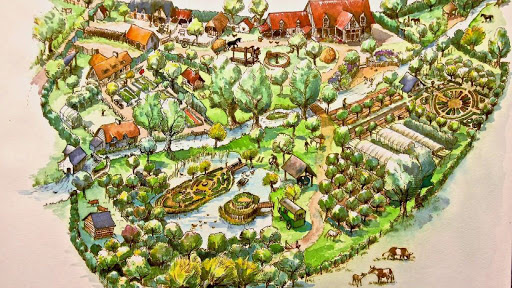
\includegraphics[height=4.15cm]{img/intro/intro-perma-culture}
    %	\caption{Ferme du Bec Hellouin}
    %\end{figure}
    
    %\paragraph{Agriculture de précision} :
    %Ce type de production se focalise sur l'utilisation de nouvelles technologies et outils numérique \cite{longaretti:hal-03233585}. Les données issues de capteurs (par ex : optique) embarqués dans des engins (machines, robots, drones, avions, satellites) permettent de recueillir des informations géo-référencées des parcelles. Grâce à un suivi régulier des parcelles, l'agriculteur a alors les moyens de piloter ses interventions localement. La parcelle n'est plus une entité homogène mais présente de nombreuses variabilités que l'on peut quantifier et cartographier. Permettant ainsi de moduler les doses d'intrants chimiques (engrais, phyto) grâce à des machines dotées d'automatisme \cite{deguine2021integrated}.
    % \og bonne dose, au bon endroit et au bon moment \fg par la prise en compte de la variabilité spatial et l'états des cultures.
    
    %\begin{itemize}
    %	\item En dépit de trois versions successives, les plans Ecophyto se sont soldés par une augmentation des quantités de produits chimiques de \SI{25}{\percent} \cite{deguine2021integrated}. % \cite{LeMondePesticides}.
    %	% Et a quasiment doublé entre 1990 et 2018, passant de 2,3 à 4,1 millions de tonnes dans le monde \footnote{\url{http://www.fao.org/faostat/en/#data/RP/visualize}}.
    %	\item Quel cout environnemental lier a l'énergie, les batterie, les métaux rares nécessaires a l'informatisation a grand échelle de l'agriculture de précision ? \cite{longaretti:hal-03233585}
    %	% https://www.youtube.com/watch?v=b8yL-ikvszE&list=PLp4dSGQ6kMnHnMvVjvA7_FpVTrMo5R6PK&index=6
    %\end{itemize}
    
    %\par Différents modèle ce confrontes donc, entre toujours plus de technologie et un changement de paradigme. Ici dans le cadre de cette thèse, nous nous intéressons au apport de l'agriculture de précision basée sur des technologies innovantes et performantes. % C'est le mode de production étudier dans notre équipe à l'UMR agroécologie et promus en partie par les plans EcoPhyto, ainsi une section dédiée en fait la présentation en \ref{sec:precise-agriculture}.
    
    \newpage
    \subsection{Transition agroécologique}
    
    Les modes de production alternatifs précédemment énoncés ont pour but de répondre à ces problématiques, tout en satisfaisant les besoins alimentaires des populations. Néanmoins, à l'exception de la permaculture, ces alternatives commencent à avoir recours aux fertilisants pour augmenter les rendements et ainsi répondre à la demande des consommateurs. Certains équilibres peuvent s'avérer difficiles à trouver, entre production et écologie, notamment pour ce qui concerne la gestion des adventices \cite{bajwa2019sustainable}. Un recours au labour retarde la levée des adventices, mais s'avère préjudiciable à la vie biologique des sols \cite{lemtiri2016crop}. Les approches dites de conservation (abondon du travail du sol profond, couverture permanente du sol, allongement des rotation) reposent sur l'usage d'herbicides de synthèse, qui ont un impact négatif sur les milieux naturels et la santé des consommateurs (comme vu dans la partie \ref{sec:02-limit-of-intensive-agriculture}) mais permettent de diminuer le compactage des sols. Pour définir une agriculture plus respectueuse de l'environnement, d'autres approches existent comme l'agroécologie et l'agriculture de précision.
    %\textcolor{red}{rmq: dernière phrase à revoir/discuter}
    %\textcolor{blue}{rmq: Je trouve maladroit de présenter l'ACS comme négative alors que cette agriculture est en pleine essor avec l'utilisation des TCS  pas de labour, semis direct, allongement rotation et  + couverture permanente des sols}
    
    %! \colorbox{orange}{permaculture ici ?}
    
    \paragraph{L'agroécologie} vise à développer une agriculture durable, en considérant les parcelles agricoles comme des agroécosystèmes. Elle s'appuie fortement sur l'utilisation de services écosystémiques \cite{altieri1999ecological, Lamarque2014, perrette2018services, lefloch2018premiere, altieri2018agroecology, haan2021designing}. Elle étudie pour cela les interactions au sein de ces écosystèmes (plantes-plantes et plantes-microorganismes) à différents niveaux d'intégration (de la molécule à la communauté) et d'échelles spatio-temporelles (microcosme, parcelle, paysage, cycle de culture, rotation, \dots).
    
    \paragraph{L'Agriculture de précision} se focalise sur l'utilisation de nouvelles technologies et outils numériques, qui permettent de recueillir des informations intra-parcellaires géo-référencées. La parcelle n'est plus considérée comme une entité homogène, mais présente une variabilité importante qui peut être mesurée et cartographiée. Grâce à un suivi régulier, l'agriculteur a alors les moyens de piloter ses interventions localement, et de réduire ses doses d'intrants chimiques (engrais, produits phytosanitaires) grâce à des machines dotées d'automatismes. L'agriculture de précision peut être une approche pour le développement de systèmes de culture à bas intrants et l'application de nouveaux produits de traitement (tels que les produits de bio-contrôle). À ce titre, elle constitue un levier pour la transition agroécologique.
    
    Plusieurs approches co-existent donc, entre culture en équilibre avec son environnement, et approche technologique visant à maîtriser les volumes d'intrants. Cette thèse s'intéresse à l'agriculture de précision telle qu'étudiée par l'UMR 1347 Agroécologie, promue par les plans Ecophyto et repose sur une gestion localisée des adventices, pour une transition agroécologique.
    % Ainsi une section dédiée en fait la présentation dans la section suivante.
    %!C.Gée -> deja dit
    % Le travail effectué dans cette thèse repose sur une gestion localisée des adventices et s'inscrit également dans le cadre d'une transition agroécologique.
    
    \newpage
    
    \section{Agriculture de précision}
    \label{sec:precise-agriculture}
    
    %! JNP
    Le concept d'agriculture de précision est apparu dans les années 80 aux États-Unis, avec la naissance des systèmes de localisation par satellite (GPS/GNSS), avec comme première application la modulation de la fertilisation en fonction des besoins des cultures \cite{robert2002precision}. \cite{mcbratney2005future, taylor2005general} définissent le concept d'agriculture de précision comme la mise en place d'une stratégie de gestion de l'ensemble de l'exploitation s'appuyant sur les technologies de l'information dans le but d'améliorer la production agricole tout en limitant l'impact environnemental. Pour ce faire, l'agriculture de précision se base sur l'étude de la variabilité intra-parcellaire, que ce soit au niveau spatial ou temporel \cite{pierce1999aspects}. En 2019, la communauté scientifique internationale  en agriculture de précision (ISPA) s'est de nouveau concertée pour proposer une nouvelle définition du terme agriculture de précision :
    
    %\par Le développement des technologies de l'information et de la communication dans la fin du 20ième siècle a aidé la mise en place de stratégie de gestion des champs de culture. C'est le début de l'agriculture de précision qui implique l'intégration de nouvelles technologies, tel-que les systèmes d'information géographique (SIG), les systèmes de positionnement globaux (GPS). L'essor de la télédétection et de la proxi-détection couplant différents capteurs entre eux a permis un niveau d'analyse des données beaucoup plus précis, permettant de révéler les variabilités intra-parcelles. En 2019, la communauté scientifique internationale lors de la conférence IPCA s'est de nouveau concertée pour proposer une nouvelle définition du terme agriculture de précision :
    
    \par \og Precision Agriculture is a management strategy that gathers, processes and analyzes temporal, spatial and individual data and combines it with other information to support management decisions according to estimated variability for improved resource use efficiency, productivity, quality, profitability and sustainability of agricultural production \fg
    
    Les technologies de l'information occupent une place fondamentale dans l'agriculture de précision \cite{lherbier2005valorisation}. La gestion localisée des parcelles peut être représentée par un cycle composé de 4 étapes (figure \ref{fig:02-intro-agri-precision-context}) : (i) l'observation des parcelles (collecte de données), (ii) la caractérisation des parcelles (traitement des données), (iii) la préconisation (prise de décision) et (iv) l'action (application au champ). Le géo-référencement (association de coordonnées géographiques aux objets étudiés) relie ces étapes entre elles.
    
    \vfill
    \begin{figure}[H]
        \centering
        %\rotatebox{90}{\scriptsize (source : \cite{lherbier2005valorisation})}
        %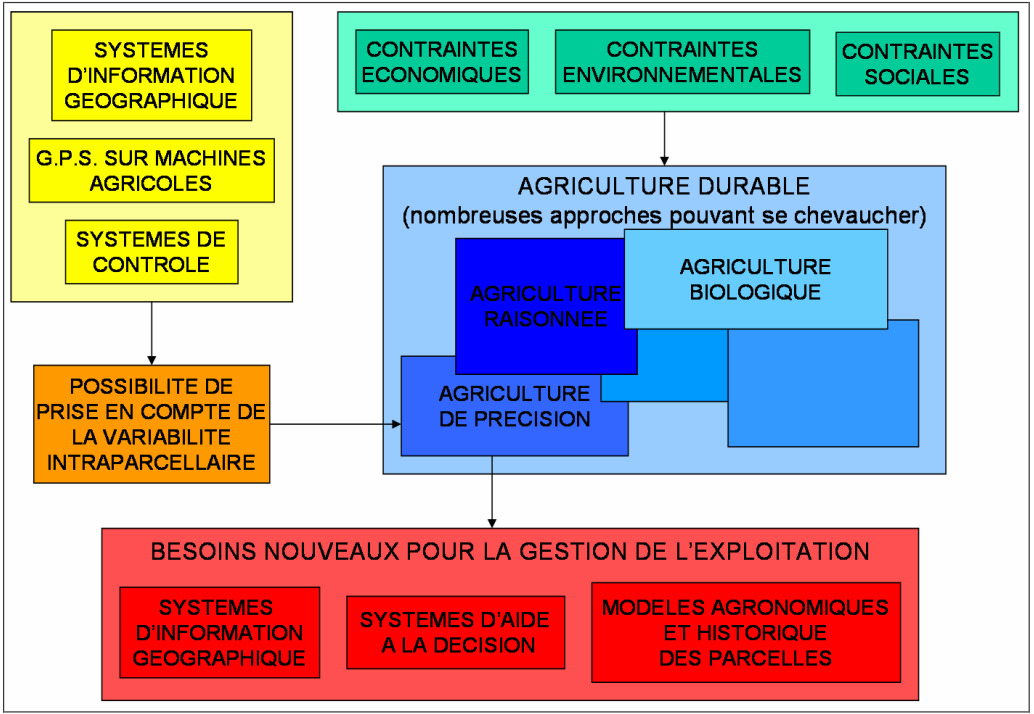
\includegraphics[height=7cm]{img/intro/intro-agri-precision-context}
        \tikzset{
	base/.style = {
		rectangle, rounded corners,
		draw=black,
		top color=white,
		bottom color=black!20,
		minimum width=3.5cm,
		minimum height=1.0cm,
		text centered,
		font=\ttfamily
	},
	every node/.style={
		font=\ttfamily,
		scale=0.8
	},
	% Specifications for style of nodes:
	activityStarts/.style = {
		base,
		fill=blue!30,
		bottom color=blue!20,
	},
	startstop/.style = {
		base,
		fill=red!30
	},
	activityRuns/.style = {
		base,
		fill=green!30
	},
	process/.style = {
		base,
		%minimum width=2.5cm,
		fill=orange!15,
		bottom color=green!20,
		font=\ttfamily
	},
	%
	point/.style={coordinate},
	draw=black!75,
	tip/.style={->,shorten >=0.007pt},
	every join/.style={rounded corners},
	align=center,
}

\begin{tikzpicture}[
	>={Latex[width=2mm,length=2mm]},
    >=latex,thick,
    node distance=1.5cm,
  ]
  \node (IMG)      [process]                {Acquisition};
  \node (GPS)      [activityStarts, below of=IMG, yshift=-0.5cm]  {Géoréférencement};
  \node (PRE)      [process, below of=GPS, yshift=-0.5cm]  {Préconisation};
  
  \node (USE)    [process, right of=GPS, xshift=-7cm, minimum height=1.2cm] {Application\\ au champ};    
  \node (PST)    [process, left of=GPS, xshift=7cm, minimum height=1.2cm] {Traitement \\ des données};
  
  \begin{scope}[->,decoration={post length=4pt},rounded corners=2mm]
  \draw[->]     (IMG) -| (PST);
  \draw[->]     (PRE) -| (USE);
  \draw[->]     (PST) |- (PRE);
  \draw[->]     (USE) |- (IMG);
  
  \draw[<->]     (GPS) -- (IMG);
  \draw[<->]     (GPS) -- (PST);
  \draw[<->]     (GPS) -- (USE);
  \draw[<->]     (GPS) -- (PRE);
  \end{scope}
\end{tikzpicture}
        \caption{Cycle de l'agriculture de précision composé de 4 étapes}
        \label{fig:02-intro-agri-precision-context}
    \end{figure}
    \vfill
    
    Ainsi, l'agriculture de précision, par le biais des nouvelles technologies \cite{app11135911}, propose par exemple une gestion intra-parcellaire de la fertilisation des cultures ou encore une gestion spécifique (SSWM Site-Specific Weed Management \cite{lopez2011weed}) de la flore adventice au plus près grâce à des systèmes de très haute précision. Les données de la parcelle sont acquises régulièrement permettant également d'utiliser des modèles agronomiques afin de proposer des prédictions pour anticiper la gestion d'une parcelle (prévision de la croissance des adventices \cite{9448338}). De plus le géo-référencement de l'information et l'utilisation de GPS haute précision, permet un guidage automatique pour moduler les doses en fonction de la variabilité spatiale \cite{PEREZRUIZ2021299}. % L'utilisation et le couplage de l'ensemble de ces outils numériques à conduit à l'émergence d'un nouveau domaine : l'agriculture numérique. L'ensemble de ces informations conduiront à formuler des outils d'aide à la décision pour accompagner les agriculteurs dans leurs interventions sur les parcelles en temps réel \cite{bellon2019avant}. L'agriculture de précision peu être vue comme une extension de l'agriculture durable.
    
    \newpage
    
    \subsection{La télédétection au service de l'agriculture de précision}
    %\subsection{Les Systèmes d'Information Géographique}
    %\subsection{Acquisition des données}
    
    La photogrammétrie aérienne fait son apparition en 1919. Des applications agricoles sont rapidement envisagées, notamment en sylviculture. \href{http://www.fao.org/3/x5339f07.htm}{En 1929, au Canada}, cette technologie permet notamment, de comptabiliser le nombre d'arbres plus rapidement qu'avec un comptage au sol et plus précisément qu'avec une estimation basée sur la surface d'exploitation. Par la suite, le développement de la stéréo-photogrammétrie permet de reconstruire de larges zones d'observations, des courbes de niveau des terrains, et cela, avec une précision métrique. Les possibilités se sont enrichies au fil des années avec le développement des appareils photo numériques et de l'imagerie satellitaire à travers la télédétection :
    
    \begin{itemize}[noitemsep]
        \item En 1962 l'US Air Force développe et lance KH-4. Deux caméras sont embarquées qui permettent de réaliser des images tridimensionnelles avec une résolution spatiale de 60 mètres. %Ils seront lancés jusqu'en 1972 à des fins d'espionnages.
        \item En 1972 les États-Unis lancent le programme Landsat ses premiers objectifs étaient l'évaluation des volumes de récolte céréalières en URSS et aux États-Unis afin d'anticiper l'évolution des cours. Le dernier, Landsat 9, a été lancé le 27 septembre 2021.
        \item En 2002, c'est au tour de agence spatiale européenne de lancer son propre satellite d'observation ENVISAT (ENVIronment SATellite) dont l'objectif est de mesurer de manière continue à différentes échelles les principaux paramètres environnementaux de la Terre relatifs à l'atmosphère, l'océan, les terres émergées et les glaces. C'est aussi le début de l'utilisation de la spectro-radiométrie permettant d'obtenir des images hyperspectrales.
        \item En 2014, c'est le programme Copernicus avec les satellites Sentinel, lancé en Europe. L'accès aux données des satellites est libre et gratuit. Le premier modèle fourni des images à 10 mètres de résolution sur plusieurs bandes spectrales. Ces très hautes résolutions permettent d'échantillonner et d'estimer différents indices sur de larges zones agricoles. Le programme Copernicus est prévu jusqu'en 2029.
    \end{itemize}
    
    Parallèlement à l'imagerie satellite, le développement de drones aériens pour l'observation a été initié pour des usages militaires. C'est dans les années 2000 que les premiers usages agricoles des drones font leurs apparitions, dont le gain en autonomie, précision, résolution ($\SI{<10}{\cm}$) et temps d'acquisition sont bien plus compétitifs que les satellites, en particulier a l'échelle de la parcelle  \cite{lherbier2005valorisation,bossu2007segmentation, Koot891024465110, Pretto2019}. La Figure \ref{fig:02-landsat} montre l'évolution de la résolution spatiale.
    
    \begin{figure}[H]
        \centering
        {\scriptsize (source : \cite{Shunlin20121})} \\
        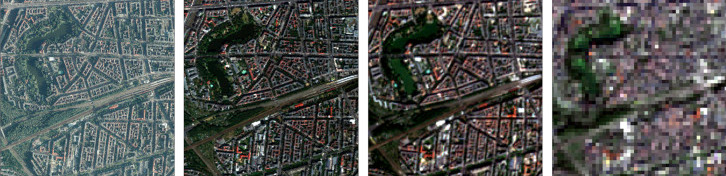
\includegraphics[width=0.7\linewidth]{img/intro/landsat} \\
        {\scriptsize Drone \SI{0.2}{\meter} \hspace{1.2cm} Avion \SI{3.6}{\meter} \hspace{1cm} Sentinel2 \SI{10}{\meter} \hspace{1cm} Landsat8 \SI{30}{\meter}}
        \caption{Évolution de la résolution spatiale}
        \label{fig:02-landsat}
    \end{figure}
    
    Les recherches en cours tendent à ajouter un degré de précision supplémentaire allant jusqu'à une résolution millimétrique. Là où les satellites et les drones aériens présentent une résolution insuffisante, ces travaux se concentrent sur le développement de l'imagerie de proxi-détection, embarquée sur machines agricoles usuelles ou sur drones terrestres \cite{machleb2020sensor}.
    
    \newpage
    %\subsection{Décision}
    \paragraph{Apport de la géomatique} Avec l'apparition de l'informatique, c'est dans les années 1960 que la géomatique fait son entrée et que le premier véritable SIG opérationnel est conçu à Ottawa, au Canada par le ministère des forêts. Afin d'obtenir des informations sur géographiques les sols, l'agriculture, la faune, la flore, et la sylviculture. La géomatique appuyée par des observations agronomiques permet de définir de premiers leviers d'intervention pour l'agriculteur \cite{lherbier2005valorisation}. La géomatique, c'est avant tout une méthodologie, en trois points :
    
    \begin{enumerate}[noitemsep]
        \item \textbf{L'observation} qui consiste à mettre en évidence et à caractériser la variabilité spatiale inter-parcellaire. Cela consiste à collecter de l'information sur le milieu et les plantes pour mieux connaître les hétérogénéités et les échanges.
        \item \textbf{L'analyse} des données pour comprendre cette variabilité, étudier l'influence de différents facteurs sur une variable et l'étude des impacts de cette variabilité sur l'opération culturale à réaliser afin d'établir les incidences économiques et environnementales.
        \item \textbf{L'action}, c'est définir avec l'agriculteur les moyens d'action et moduler ces pratiques en fonction de l'itinéraire technique qu'il souhaite mettre en œuvre.
    \end{enumerate}
    
    La géomatique, travail donc a l'échelle du territoire (bassin versant, vallée, région, \dots), c'est-à-dire les interactions entre différentes parcelles et les mouvements de flux tels que les polluants, les sédiments ou autres. Tous ces facteurs ont un rôle important à ces grandes échelles par exemple sur les rendements et la biodiversité comme nous l'avons vus précédemment. Ainsi des modèles d'agencement sont modélisables (figure \ref{fig:02-simulation}) permettant d'optimiser les rendements à l'échelle du territoire \cite{caquet2020agroecologie}. 
    
    \begin{figure}[H]
        \centering
        \rotatebox{90}{\scriptsize (source : \cite[p.~74]{caquet2020agroecologie})}
        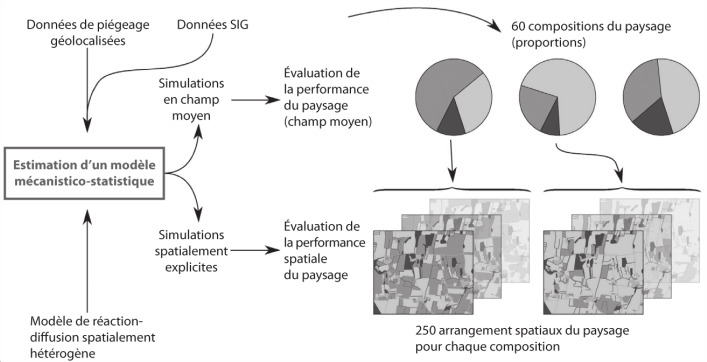
\includegraphics[height=8cm]{img/intro/simulation}
        \caption{Simulation de l'agencement spatial de paysages}
        \label{fig:02-simulation}
    \end{figure}
    
    En augmentant la résolution de ces observations, des modèles de simulation des interactions entrent les plantes ont commencé à voir le jour pour montrer l'influence de différents facteurs sur l'ensemble du système (itinéraire technique, adventice, \dots) à l'échelle de la parcelle, tel-que FLORSYS \cite{colbach2021florsys}. Ces méthodes ont donc permis de passer d'une gestion des doses (intrant, phytosanitaire, \dots) de l'exploitation (homogène et uniforme), à un traitement des zones ``dégradées'' de la parcelle après analyse \cite{lherbier2005valorisation}. 
    %! On comprend ici, que la géomatique est le fondement de l'agriculture de précision. 
    
    
    
    %Certaines de ces analyses ont pu être transposer a l'échelle de la parcelle par exemple avec des analyses de conductivité du sol montrent une variabilité de substrat et donc de rendement a l'échelle de la parcelle \cite{luck2009electrical}, cette variabilité intra-parcellaire est utilisée avec succès pour moduler l'apport de fertilisant, par le biais d'une carte géo-référencé et de modulation des systèmes d'épandages.
    
    %
    
    %\par Ces méthodes ont donc permis de passer d'une gestion des doses (intrant, phytosanitaire, \dots) de l'exploitation (homogène et uniforme), à un traitement des zones ``dégradé'' de la parcelle après analyse \cite{lherbier2005valorisation}. C'est précisément l'agriculture de précision, qui reconnaît donc une variabilité spatial associer aux caractéristiques locale du sols (texture, fertilité, \dots) et l'états des cultures (adventices, stress, insectes, champignon), impliquant la recherche des problème, leurs localisation et délimitation pour une gestion locale. Dans le cas d'infestation par les adventices, leurs types, position et étendue sont alors cartographiées, puis utilisées pour appliquer l'herbicide approprié avec la \og bonne dose, au bon endroit et au bon moment \fg.
    
    \newpage
    \subsection{Vers une agriculture numérique}
    \label{sec:numerical-agriculture}
    
    % https://www.smart-akis.com/index.php/fr/reseau/quest-ce-que-l-agriculture-numerique/
    Parallèlement au développement de l'agriculture de précision, de nouvelles technologies ont récemment émergé : réseaux de télécommunication, internet des objets \cite{TANG2021105895}, fouille de données, apprentissage profond et intelligence artificielle . L'utilisation et le couplage de l'ensemble de ces outils numériques conduit à l'émergence d'un nouveau domaine : l'agriculture numérique \cite{Birner2021}.
    Les applications envisagées reposent sur l'utilisation de multiples capteurs qui peuvent être embarqués dans plusieurs drones \cite{Pretto2019}. Ainsi, un drone terrestre peut être piloté à partir d'images acquises par des drones aériens. (figure \ref{fig:02-agri-precision}). Une communication entre modules est alors nécessaire.
    
    %Ces approches reposes sur l'utilisation de multiple-capteurs et peuvent mobilisé plusieurs drones. Ainsi le drone terrestre peut être aidé par des analyses faites par drones aérien, avec une gestion de l'altitude (figure \ref{fig:02-agri-precision}) et une communication entres modules est alors nécessaire. L'agriculture numérique utilise donc des réseaux intelligents pour récupéré de l'information en temps réelle de multiples modules et capteurs. C'est donc une extension de l'agriculture de précision.
    
    \vfill
    \begin{figure}[H]
        \centering
        {\scriptsize (source : \cite{Pretto2019})} \\
        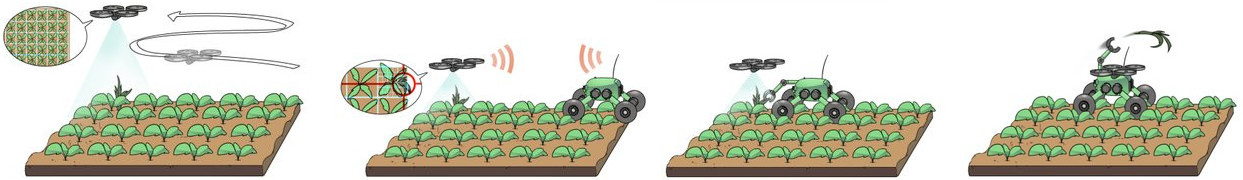
\includegraphics[width=\linewidth]{img/intro/agri-precision-flat}
        \caption{Concept de projet en agriculture numérique}
        \label{fig:02-agri-precision}
    \end{figure}
    \vfill
    
    L'ensemble des informations collectées permettent de constituer des outils d'aide à la décision pour accompagner les agriculteurs dans leurs interventions sur les parcelles en temps réel \cite{bellon2019avant, saddik2022computer}. Il est ainsi possible d'envisager : %L'identification des plantes aux champs, d'appliquer des fertilisants au plus près des cultures, d'éliminer les plantes indésirables tout en préservant si possible les plantes présentant des services écosystémiques.
    d'identifier des plantes au champs (espèce, stade de développement), d'appliquer des produits phytosanitaires au plus près des cultures, ou d'éliminer les plantes indésirables tout en préservant les plantes présentant des services écosystémiques \cite{Green2021}.
    
    %! JNP
    \paragraph{Lien avec l'agroécologie} : L'agriculture de précision, et par extension l'agriculture numérique peuvent permettre de réduire l'impact environnemental des différents traitements précédemment présentés (herbicides, fongicides, insecticides, fertilisants, \dots), en diminuant les surfaces traitées et les doses appliquées. Les problématiques liées au tassement des sols seront grandement amoindries, puisque ce type d'approche peut être embarqué sur de ``petits'' robots autonomes, plus légers. Malgré tout, ces approches restent pour l'instant hyper-spécialisées et ne laissent donc que peu de place à l'hétérogénéité des cultures, ce qui implique que les processus agroécologiques (interactions biotiques, services écosystémiques) ne sont pas encore mobilisables \cite[p.~81]{caquet2020agroecologie}.
    
    %Dans un premier temps ont cherche a réduire l'impacte environnemental des différents traitements précédemment présenté, en diminuant leurs utilisations (micro-dose) tel-que les herbicides, pesticides et fertilisants, et donc le coût de ces derniers aux près des agriculteurs. Bien que le but, à terme, est la suppression des produits phytosanitaires par l'utilisation d'autres méthodes dites écologiques en ne remplaçant que la parti ``pulvérisation'' du système. Finalement les problématiques précédemment exposées et liées au lessivages des sols seront grandement amoindri, puisque ce type d'approches peu être embarquées sur de ``petit'' robot autonome, limitant le compactage des sols. Malgré tout, ces approches restent hyper-spécialisées et ne laisse donc peu de place a l'hétérogénéités des cultures, ce qui implique que ces processus agroécologiques ne sont pas encore mobilisables \cite[p.~81]{caquet2020agroecologie}.
    
    \paragraph{Phénotypage} : A contrario cette hyper-spécialisation n'est pas un frein dans le domaine du phénotypage à haut débit. Cela permet d'accélérer les progrès dans la sélection des variétés \cite{cabrera2012high}, pour répondre aux attentes des différents acteurs en augmentant la rapidité d'acquisition des mesures, qui sont de plus non-destructives \cite{jiang2020convolutional}. C'est le cas par exemple de la culture d'igname, dont le manque de variétés améliorées sur le rendement et les attributs de qualité, entraînent un déclin de la filière aux Antilles et freinent l'adoption de nouvelles variétés en Afrique de l'Ouest. L'objectif est de quantifier le rendement par la dynamique de recouvrement, la qualité ``subjective'' est associée à la couleur de la chair des tubercules et son oxydation dans le temps. La qualité nutritionnelle des produits à base d'igname, peut être déterminée par la taille et la forme des grains d'amidon, en utilisant l'analyse d'image \cite{mell:dumas-02138698, cornet:hal-02791432}.
    
    \newpage
    \section{Le désherbage}
    
    \subsection{Place des adventices dans les systèmes de culture}
    \label{sec:place-adventice}
    
    %\subsection{Définition d'une adventice}
    
    
    %\subsubsection{a) La gestion des adventices}
    Les adventices sont des plantes, non désirées ni semées par l'agriculteur, se développant naturellement dans un système de culture (ou agrosystème). En fonction du mode de production, les adventices font l'objet d'une attention particulière. Nous resterons à partir de maintenant dans le cadre de l'agriculture conventionnelle et de l'agriculture de précision.
    
    \par Dans ce contexte, depuis le début du XXe siècle, les adventices sont considérées comme indésirables car responsables de la perte de rendement et de qualité \cite{cordeau2016nuisibilite}. On parle dans ce cas, de nuisibilité primaire \cite{caussanel:hal-00885190}. Elle se mesure avec le nombre de pieds d'adventices par m² qui occasionne une baisse de rendement de \SI{5}{\percent} en système conventionnel. Cependant, ce paramètre de densité de plantes a été remis en cause, car il ne prend pas en compte le stade de la végétation. C'est pourquoi de nouveaux paramètres ont été proposés comme le ratio de biomasse entre adventices et cultures (BMw/BMc), ou en étudiant le rapport des surfaces foliaires, plus simple à caractériser par des méthodes non-destructives \cite{Gee2021}. La nuisibilité secondaire concerne les conséquences engendrées sur la parcelle sur le long terme (stock semencier, salissement, etc).
    
    \par Pour acquérir une compréhension fiable des risques de réduction des récoltes dans le temps, des expériences acquises localement dans des conditions comparables sur 110 essais de contrôle des adventices ont été menées en France entre 1993 et ​​2015 sur trois grandes cultures annuelles (blé tendre, colza et tournesol). Des réductions de \SI{25}{q\per\hectare}, \SI{4}{q\per\hectare} et \SI{3,5}{q\per\hectare} ont respectivement été observées \cite{cordeau2016nuisibilite}. Les adventices rivalisent donc avec leurs plantes voisines par une concurrence accrue pour les nutriments (azote, potasse, phosphore), la lumière et l'eau. La nuisibilité des adventices reste un sujet d'étude par la communauté scientifique. Comprendre la compétition des adventices avec la culture pour les ressources du milieu (lumière, eau, nutriments, \dots) est très complexe du fait d'une interaction multi-spécifique et qui dépendra du stade de développement des plantes \cite{morison2008comment, colbach2021florsys}. Toutefois, d'autres études, suggèrent qu'il existe un manque de connaissances concernant la ``réelle'' nuisibilité pour les cultures \cite{bendaoud2020semis, jouan:hal-03611906}.
    
    \par A travers cette complexité, la conséquence pratique d'une telle gestion devient donc pour les agriculteurs de trouver des solutions globales simples et pratiques de mise en œuvre ; c'est ce que la chimie de synthèse a pu apporter avec des herbicides systémiques (à large spectre) ou spécifiques (pour une espèce particulière). Cependant, certaines adventices offrent par exemple des services écosystémiques (figure \ref{fig:02-adventice-service}), d'autres sont comestibles (figure \ref{fig:02-adventice-comestible}) et enfin certaines sont plus ou moins ``toxiques'', mais peuvent trouver des usages médicinaux (figure \ref{fig:02-adventice-toxique}).
    
    
    
    % https://ree.developpement-durable.gouv.fr/themes/risques-nuisances-pollutions/pollution-de-l-eau-douce/pesticides/article/l-indice-pesticides-dans-les-cours-d-eau
    
    %\begin{figure}[H]
    %	\centering
    %	% http://www.ipreunion.com/volcan/reportage/2018/03/28/un-rapport-accablant-des-pesticides-dans-la-quasi-totalite-des-eaux-reunionnaises,79264.html
    %	\rotatebox{90}{\scriptsize (source : wikipedia.fr) }
    %	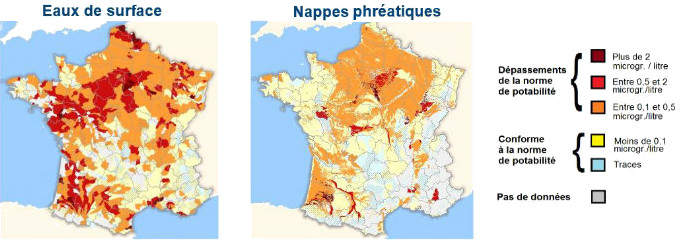
\includegraphics[height=5cm]{img/intro/intro-carte-pesticide}
    %	\caption{Presence de pesticide dans la majorités des cours d'eau}
    %	\label{fig:02-intro-carte-pesticide}
    %\end{figure}
    \newpage
    \null \vfill
    
    \begin{figure}[H]
        \centering
        {\scriptsize (source : flora-electronica)} \\
        \begin{subfigure}{0.2\linewidth}
            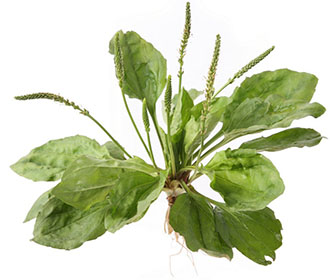
\includegraphics[height=3cm]{img/intro/plante-plantain.jpg}
            \caption{plantain}
        \end{subfigure}
        \hspace{1cm}
        \begin{subfigure}{0.2\linewidth}
            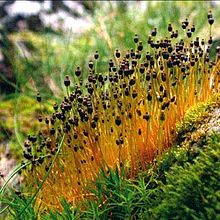
\includegraphics[height=3cm]{img/intro/plante-bryophyte.jpg}
            \caption{bryophyte}
        \end{subfigure}
        \hspace{1cm}
        \begin{subfigure}{0.2\linewidth}
            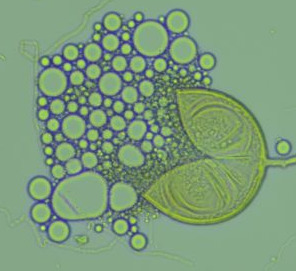
\includegraphics[height=3cm]{img/intro/plante-mycorrhiza}
            \caption{mycorhize}
        \end{subfigure}
        \caption{Plantes bio-indicatrices, fixatrices et symbiotiques}
        \label{fig:02-adventice-service}
    \end{figure}
    
    Certaines adventices aident par exemple, à la structuration du sol, à la réduction des phénomènes érosifs, à l'absorption des excédents de fertilisation et sont des indicateurs d'un état particulier du milieu comme le plantain. D'autres permettent la fixation de l'azote tels que les bryophytes et des champignons augmentant significativement les rendements avec les mycorhizes \cite{zerbib2018relations}. Elles participent également à la diversité écologique du milieu en servant de refuge et en pourvoyant des ressources alimentaires (pollen, nectar) aux auxiliaires des cultures \cite{schaub2010mieux, morison2008comment}.
    
    \begin{figure}[H]
        \centering
        {\scriptsize (source : flora-electronica)} \\
        \begin{subfigure}{0.2\linewidth}
            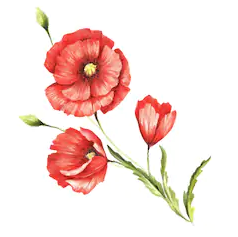
\includegraphics[height=3cm]{img/intro/plante-coquelicot.jpg}
            \caption{coquelicot}
        \end{subfigure}
        \hspace{1cm}
        \begin{subfigure}{0.2\linewidth}
            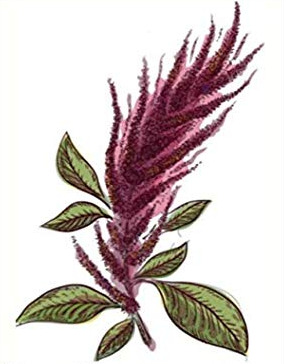
\includegraphics[height=3cm]{img/intro/plante-amarante}
            \caption{amarante}
        \end{subfigure}
        \caption{Adventices comestibles}
        \label{fig:02-adventice-comestible}
    \end{figure}
    
    Certaines sont également comestibles et des phénomènes de résistance aux herbicides ont commencé à émerger.
    C'est le cas du coquelicot en France et de l'amarante aux USA due à la sur-utilisation d'herbicide et entraînant des mutations.
    
    \begin{figure}[H]
        \centering
        {\scriptsize (source : flora-electronica)} \\
        \begin{subfigure}{0.2\linewidth}
            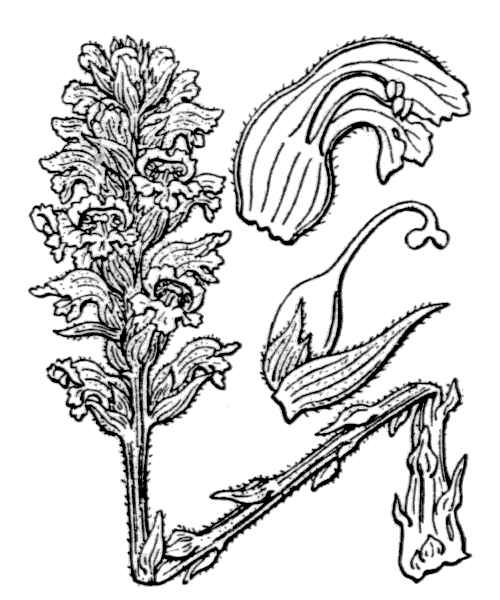
\includegraphics[height=3cm]{img/intro/plante-orobanche.jpg}
            \caption{orobranche}
        \end{subfigure}
        \hspace{1cm}
        \begin{subfigure}{0.2\linewidth}
            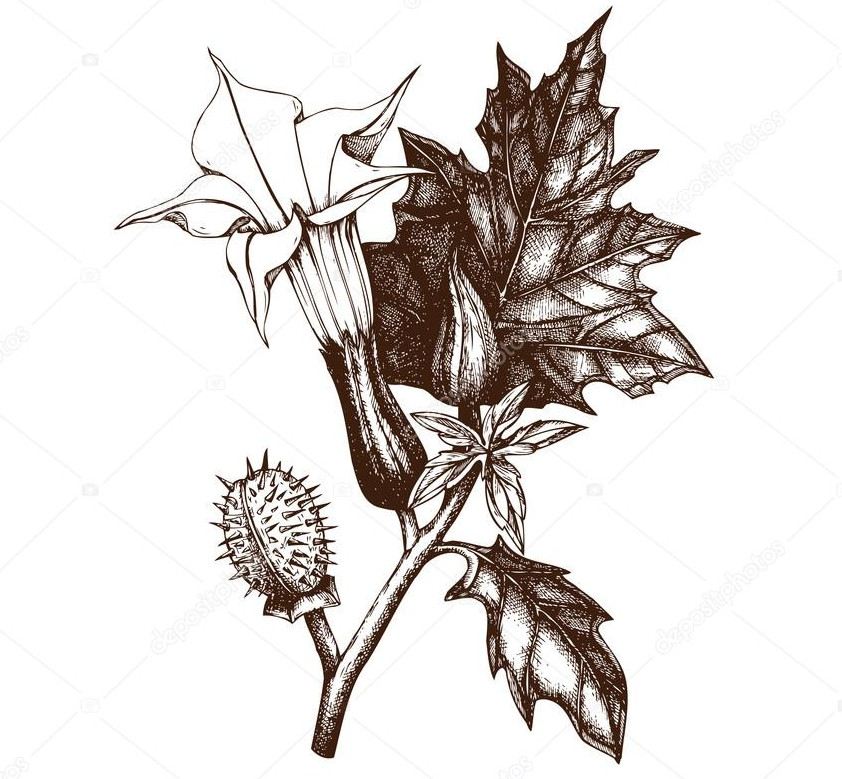
\includegraphics[height=3cm]{img/intro/plante-stramoine.jpg}
            \caption{stramoine}
        \end{subfigure}
        \hspace{1cm}
        \begin{subfigure}{0.2\linewidth}
            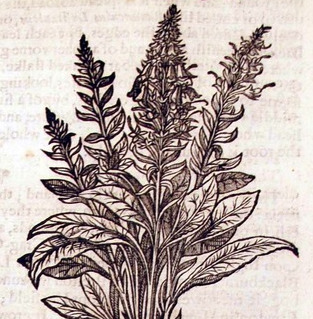
\includegraphics[height=3cm]{img/intro/plante-digitale}
            \caption{digitale}
        \end{subfigure}
        \caption{Adventices parasite, psychotrope et médicinal}
        \label{fig:02-adventice-toxique}
    \end{figure}
    
    \par Certaines adventices ont toutefois des inconvénients importants. C'est le cas de l'orobanche, une plante parasite qui utilise les nutriments de l'hôte, du stramoine plante chamanique fortement présente dans le maïs et qui provoque des délires. Ainsi que de la digitale qui est une plante médicinale à très faible dose.
    %SICARD, Hélène, FONTAINE, Laurence et ZAGANIACZ, Véronique, 2012.
    %Connaître les adventices pour la maîtriser en grandes cultures sans herbicides.
    
    \vfill 
    \newpage
    \subsection{La biologie des adventices}
    
    La connaissance de la biologie des adventices est essentielle pour mettre en œuvre des stratégies de désherbage. Ceci est d'autant plus important pour les systèmes d'agriculture biologique où l'utilisation d'herbicides est interdite. Parmi les principales notions à connaître sur les adventices, il y a : la profondeur de germination (figure \ref{fig:02-iwm-depth}), l'époque préférentielle de germination (figure \ref{fig:02-iwm-seedling}) et le taux annuel de décroissance (figure \ref{fig:02-iwm-stock}) de ces adventices.
    
    \vfill
    \begin{figure}[H]
        \centering
        %{\scriptsize (source : \href{https://nord-pas-de-calais.chambre-agriculture.fr/fileadmin/user_upload/Hauts-de-France/028_Inst-Nord-Pas-de-Calais/Telechargements/Agriculture-biologique/Brochures-desherbage-dechaumage.pdf}{nord-pas-de-calais.chambre-agriculture.fr})} \\
        %{\scriptsize (source : \href{http://bhu.org.nz/future-farming-centre/9-homepage/ffc}{bhu.org.nz})} \\
        \source{d'après \cite{roberts1982weed}}
        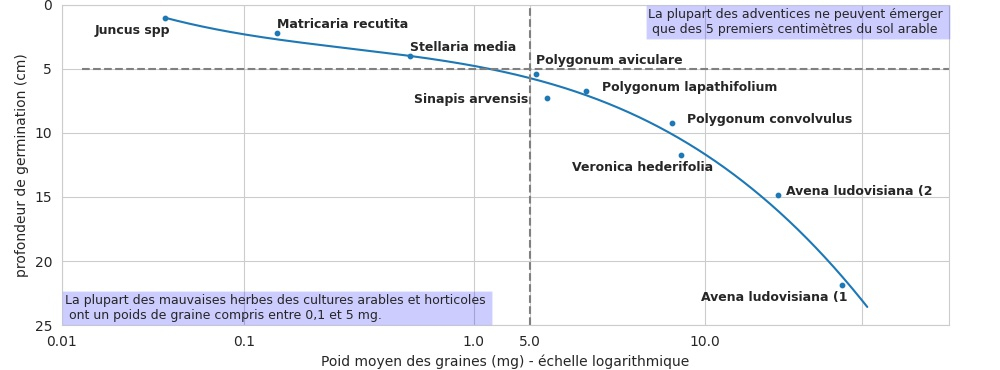
\includegraphics[width=\linewidth]{img/intro/iwm-depth-3}
        \caption{Profondeur de germination en fonction de la masse des graines}
        \label{fig:02-iwm-depth}
    \end{figure}
    \vfill
    
    Aussi, les adventices se caractérisent par une profondeur de germination préférentielle. Pour la plupart d'entre elles, la germination se produit principalement à une profondeur de moins de \SI{5}{cm}. La plupart des semences sont incapables de germer au-delà de \SI{10}{cm} de profondeur. Donc enfouir les graines en profondeur par le labour permet d'empêcher leurs levées, même si elles ont tendance à se conserver plus longtemps. Il y a cependant quelques exceptions, comme la folle avoine, une espèce à grosses graines qui peut germer au-delà de \SI{10}{cm}.
    
    \begin{figure}[H]
        \centering
        %{\scriptsize (source : \href{https://www.terre-net.fr/observatoire-technique-culturale/strategie-technique-culturale/article/connaitre-l-ennemi-pour-mieux-le-combattre-217-83255.html}{terre-net.fr})} \\
        %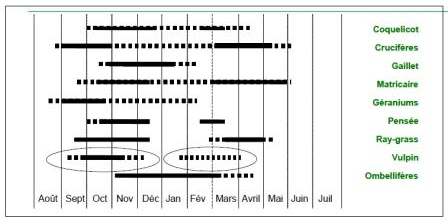
\includegraphics[width=0.7\linewidth]{img/intro/iwm-seedling}
        \source{\href{http://www.ile-de-france.chambagri.fr/pro77/rep-agronomie/agroequipement/files/160822_FicheLeviersAgro.pdf}{www.ile-de-france.chambagri.fr}}
        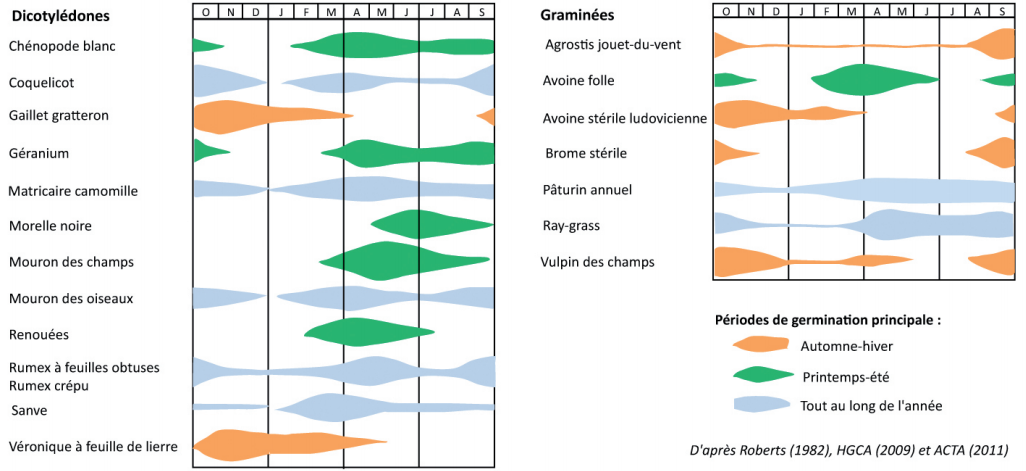
\includegraphics[width=\linewidth]{img/intro/iwm-seedling-2}
        \caption{Période préférentielle de germination de certaines adventices}
        \label{fig:02-iwm-seedling}
    \end{figure}
    
    \newpage
    \par Les adventices annuelles se caractérisent aussi par leur période de germination. Certaines adventices apparaissent sur une période relativement courte (Vulpinia, qui apparaît en automne et en hiver) ou, à l'inverse, sur une longue période, voire toute l'année (pâturin annuel). La concentration des plantations sur une période de temps limitée conduit à une spécialisation de la flore. Par exemple, les systèmes dominés par les cultures d'hiver (colza-blé) favorisent le développement des adventices d'automne-hiver comme Vulpinia. \\
    
    \vfill
    \begin{figure}[H]
        \centering
        {\scriptsize (source : \href{http://www.agro-transfert-rt.org/wp-content/uploads/2016/02/Des_parcelles_plus_propres_avec_moins_dherbicides.pdf}{agro-transfert-rt.org)}} \\
        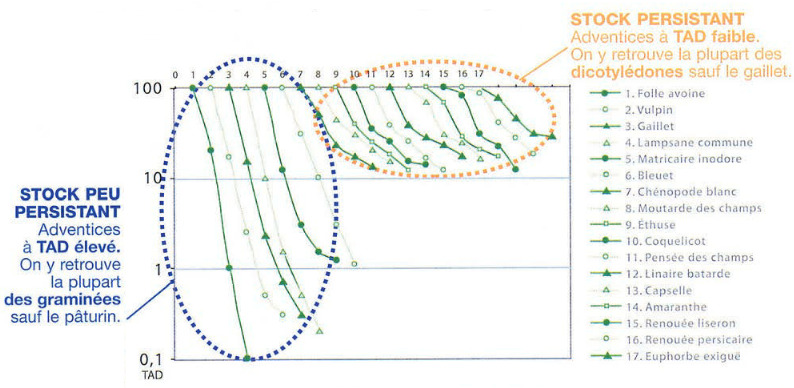
\includegraphics[width=\linewidth]{img/intro/iwm-stock}
        \caption{Taux annuel de décroissance du stock semencier des adventices}
        \label{fig:02-iwm-stock}
    \end{figure}
    \vfill
    
    \par Finalement, il y a le Taux Annuel de Décroissance (TAD) qui correspond au pourcentage de graines qui disparaissent d'une année à l'autre. Il montre l'évolution de la viabilité des graines d'adventices dans le sol. Le nombre de graines viables diminue chaque année proportionnellement à la valeur TAD. Plus le TAD est élevé, plus la durée de vie des semences est courte. Les adventices à faible TAD sont plus difficiles à contrôler, car le labour est beaucoup moins efficace pour lutter contre ce type d'adventices, puisqu'elles seront encore capables de germer lors du prochain labour. La plupart des graminées ont un TAD élevé, tandis que les graines des dicotylédones telles que le coquelicot, le chénopode ou la renouée ont une durée de vie assez longue. Ainsi, la durée de vie des graines est très variable d'une espèce à l'autre. Les graines des adventices céréalières ont une durée de vie exceptionnellement longue. Certaines on pu germer après 1700 ans \cite{wesson1967light}.
    
    
    %/ parler monocot / dicot
    %◦ adventices annuelles
    %◦ adventices biannuelles ou pluriannuelles
    %◦ adventices dites ‘vivaces', les plus difficiles à contrôler
    %Ainsi, selon les systèmes de culture étudiés, il pourrait être intéressant d'arriver à identifier les espèces les plus nuisibles, leur périodes de levées préférentielles pour identifier celles qui vont se reproduisent le plus vite pour mieux les contrôler…..
    
    \newpage
    \subsection{Fenêtres de traitement}
    
    Les moments de gestion des adventices peuvent être définis par cinq "fenêtres d'opportunité", déterminées par le cycle de la culture semée (Figure \ref{fig:02-weed-life-stages}) et le stade de vie des adventices \cite{agronomy11040747}. (fenêtre 1) Avant le semis d'une culture, les herbicides non-sélectifs et le travail du sol peuvent être utilisés pour contrôler les adventices dans le stock semencier ou les plantules émergentes. (fenêtre 2) Après le semis, mais avant l'émergence de la culture, des herbicides de pré-émergence (PRE-herbicides), des cultures de couverture ou le paillage peuvent être utilisés pour contrôler sélectivement la levée des adventices. (fenêtre 3). Les herbicides sélectifs et la lutte mécanique contre les adventices peuvent être utilisés lorsque les plantules sont suffisamment petites pour être contrôlées et avant qu'elles ne commencent à concurrencer la culture (fenêtre 4). Une fois que les adventices commencent à se disputer les ressources, l'augmentation de la compétitivité du couvert végétal peut engendrer des pertes de rendement et le retour des graines d'adventices. Enfin,les progrès récents dans le contrôle des graines des adventices après la récolte ont également soulevés la possibilité de réduire les populations d'adventices en détruisant les graines fraîches (fenêtre 5).
    
    \vfill
    \begin{figure}[H]
        \centering
        %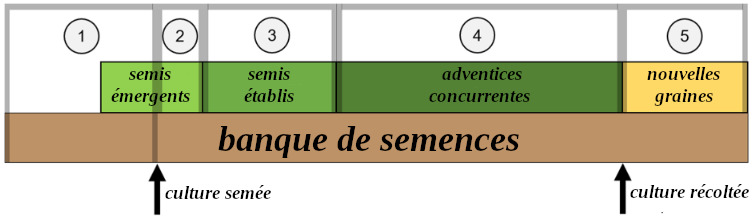
\includegraphics[width=0.76\linewidth]{img/intro/weed-life-stages}
        \begin{tikzpicture}[
    >=stealth',thick,
	point/.style={coordinate},
	every join/.style={rounded corners},
	align=center,
	%
    table nodes/.style={
        rectangle,
        draw=black,
        align=center,
        minimum height=7mm,
        text depth=0.5ex,
        text height=2ex,
        inner xsep=0pt,
        outer sep=0pt
    },      
    table/.style={
        matrix of nodes,
        row sep=-\pgflinewidth,
        column sep=-\pgflinewidth,
        nodes={
            table nodes
        },
        execute at empty cell={\node[draw=none]{};}
    },
    %
    window/.style = {
		circle,
		draw=black,
		top color=white,
		bottom color=black!20,
    },
	base/.style = {
		rectangle,
		draw=black,
		top color=white,
		bottom color=black!20,
		minimum width=4cm,
		text centered,
		font=\ttfamily
        %font=\sffamily
	},
    semis1/.style = {
        base,
        top color=green!10,
        bottom color=green!80,
        minimum height=1.25cm,
    },
    semis2/.style = {
        base,
        top color=green!25,
        bottom color=green!80!black,
        minimum height=1.25cm,
    },
    semis3/.style = {
        base,
        top color=green!40,
        bottom color=green!60!black,
        minimum height=1.25cm,
    },
    semis4/.style = {
        base,
        top color=orange!80,
        bottom color=orange!60!black,
        minimum height=1.25cm,
    },
	banque/.style = {
		base,
	    top color=orange!40!white,
	    bottom color=orange!40!gray,
		minimum height=1.2cm,
	},
	%
    tip/.style={->,shorten >=0.007pt},
	every node/.style={font=\ttfamily, scale=0.8},
]

    \draw[black,thick] (-4.0,-2.2) rectangle (11.2,0.7);

	\node (p01) [window, yshift=2mm, xshift=-30mm]  {1};
	\node (p02) [window, yshift=2mm, xshift=10mm]   {2};
	\node (p03) [window, yshift=2mm, xshift=40mm]   {3};
	\node (p04) [window, yshift=2mm, xshift=80mm]   {4};
	\node (p05) [window, yshift=2mm, xshift=120mm]  {5};
	
	
	\draw[-, line width=2mm, opacity=0.3] (00mm, 7mm) -- (00mm, -22mm);
	\draw[-, line width=2mm, opacity=0.3] (16mm, 7mm) -- (16mm, -22mm);
	\draw[-, line width=2mm, opacity=0.3] (48mm, 7mm) -- (48mm, -22mm);
	\draw[-, line width=2mm, opacity=0.3] (80mm, 7mm) -- (80mm, -22mm);
	
	\node (p11) [semis1, yshift=-10mm, xshift=0mm]   {\large semis\\[-0.2em] \large émergents};
	\node (p12) [semis2, yshift=-10mm, xshift=40mm]   {\large semis\\[-0.2em] \large établis};
	\node (p13) [semis3, yshift=-10mm, xshift=80mm]   {\large adventices \\[-0.2em] \large concurrentes};
	\node (p14) [semis4, yshift=-10mm, xshift=120mm]   {\large nouvelles\\[-0.2em] \large graines};
	
	\node (p22) [banque, fit={(-5.518,-13mm) (13.2,-22mm)}, xshift=-3mm]   {\vskip 0pt \huge banque de semences};
	
	\node (p31) [base, yshift=14mm, xshift=-30mm]  {\large Culture semée};
	\node (p32) [base, yshift=14mm, xshift=67mm]  {\large Culture récoltée};
	
	\draw[->,thick] (p31) -| (00mm, 7mm);
	\draw[->,thick] (p32) -| (80mm, 7mm);
\end{tikzpicture}
\vspace{0.5em}
        \caption{Illustration de cinq fenêtres d'opportunité pour la gestion des adventices}
        \label{fig:02-weed-life-stages}
    \end{figure}
    \vfill
    
    Les solutions de gestion reposent donc sur une connaissance approfondie du cycle de développement et cycle de reproduction \cite{chauvel2018gestion}. La rotation des cultures, le désherbage, le travail du sol et les mesures préventives sont les seuls leviers d'influence sur les populations d'adventices des parcelles. Néanmoins, les solutions de gestion des adventices favorisent les espèces qui ont le même cycle de développement et les mêmes caractéristiques (monocotylédone ou dicotylédone) que les cultures. À travers cette thèse, nous proposons un axe de recherche permettant la réduction des produits phytosanitaires. %, voir conservées les adventices présentant des avantages.
    Plus spécifiquement, dans le cadre du Challenge RoSE, nous nous intéressons aux stades de développement les plus précoces des adventices, afin d'en limiter leur développement (fenêtre 1 et 2).
    
    \par Ainsi, selon les systèmes de culture étudiés, il pourrait être intéressant d'arriver à identifier les espèces les plus nuisibles, leurs périodes de levées préférentielles pour identifier celles qui vont se reproduire le plus vite pour mieux les contrôler. % Une sélection des adventices pourrait être l'avenir de l'agriculture de précision.
    
    %=>parler de gestion intégrée (IWM) de gestion des adventices
    
    \newpage
    %\section{Les technologies de désherbage}
    
    \subsection{Les technologies de désherbage actuelles}
    
    Le pulvérisateur est la principale machine agricole utilisée pour le désherbage chimique. Ce dernier se compose d'une cuve, qui contient la bouillie (mélange eau+produit phytosanitaire) à appliquer ainsi que le système de mise sous pression du fluide, et d'une rampe d'épandage dont la bouillie sous pression circule vers les buses qui vont fragmenter le jet en gouttelettes (figure \ref{fig:02-epandage}).  Un système de régulation permet à chaque instant de contrôler le débit de pulvérisation selon l'avancement de la machine pour maîtriser le volume de bouillie épandu par hectare.
    %!C.Gée
    %Un système de régulation permet à chaque instant de contrôler le débit de pulvérisation selon l'avancement de la machine pour maîtriser le volume de bouillie épandu par hectare.
    %Pour contrôler le volume épandue par hectare, une régulation en fonction de la vitesse de la machine peut être utilisée.
    
    \begin{figure}[H]
        \centering
        \rotatebox{90}{\scriptsize (source : \cite{jones2009modelisation})}
        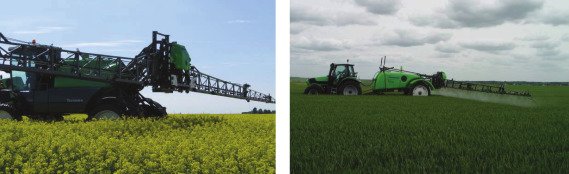
\includegraphics[width=0.6\linewidth]{img/intro/rampe-epandage} \\
        \caption{Exemple de pulvérisateurs}
        \label{fig:02-epandage}
    \end{figure}
    
    %! Ces buses permettes de fragmenter le produit en gouttelettes. Et le choix de ces
    Le choix des buses dépend de différents facteurs tels que, la viscosité du fluide, la pression, le débit, la vitesse de pulvérisation, la taille des gouttelettes et la dérive en fonction de la couverture souhaitée (figure \ref{fig:02-buses}). À noter le développement de buses anti-dérive à injection d'air, permettant de créer des gouttelettes plus grosses, et donc moins sensibles à la dérive \cite{vulga2015}. Leur utilisation permet de réduire la largeur des zones non traitées en bordure des points d'eau (de \SI{20}{\cm} ou \SI{50}{\cm} à \SI{5}{\meter}) et, sous certaines conditions, les distances non traitées à respecter vis-à-vis des riverains.
    
    \begin{figure}[H]
        \centering
        %\rotatebox{90}{\scriptsize (source : \cite{vulga2015}}
        %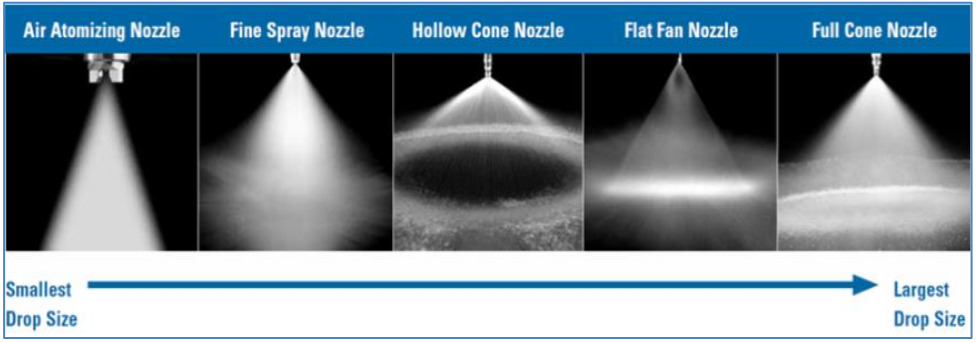
\includegraphics[width=0.7\linewidth]{img/intro/buses}
        
        \source{\href{https://www.spray-nozzle.co.uk/home/resources/engineering-resources/guide-to-spray-properties/1---introduction/spray-nozzle-questions/test}{spray-nozzle.co.uk}}
        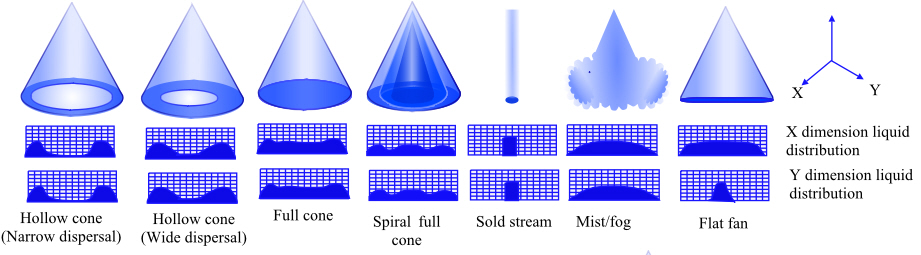
\includegraphics[width=\linewidth]{img/intro/spray-pattern-distributions.jpg} \\
        \caption{Différentes formes de buses associées}
        \label{fig:02-buses}
    \end{figure}
    
    \par Appuyés par les GPS/GNSS et la géomatique, les systèmes de pulvérisation se sont grandement améliorés afin de prendre en compte la variabilité spatiale. Ainsi, après l'observation et l'analyse des données du champ, une carte géoréférencée (dite de préconisation) est embarquée sur le pulvérisateur permettant d'agir (ON/OFF) localement grâce à des électrovannes installées sur les rampes. Ces dernières sont commandées par un ordinateur intégré (ou terminal isobus) et une communication ISOBUS : c'est ce que l'on appelle la coupure de tronçon. Permettant ainsi d'ouvrir ou non toutes les buses sans modulation. Depuis, il est possible de faire une commutation sur un porte-buse type quadri jet avec une coupure électrique permettant d'intégrer la coupure individuelle de la buse. Enfin, de nouvelles buses à pulsation (reposant sur la technologie Pulse-Width Modulation) ont fait leur apparition, permettant de faciliter le traitement localisé pour aller vers une modulation de dose.
    %\textcolor{red}{rmq: attention, le PWM permet de moduler le débit en fonction de la vitesse pour conserver une dose constante. Il permet également la modulation mais on ne module pas les apports d'herbicide (ok pour engrais et fongi)}
    
    \newpage
    
    Dans la même lignée de technologie de traitement que la pulvérisation, les systèmes de pulvérisation ponctuelle (spot spraying) ont fait leur apparition. Ce sont des appareils,  permettent de traiter ``uniquement'' l'inter-rang (tels que le WeedSeeker ou le Weed-It). Le dispositif attaché à la rampe de pulvérisation (visible en rouge sur la figure \ref{fig:02-traitement-weed-seeker}), permet de détecter la présence de végétation grâce à une photodiode et l'utilisation d'indice de végétation (présentés en section \ref{sec:vegetation-indices}). Lorsque de la végétation est détectée, l'électrovanne la plus proche est ouverte afin de traiter uniquement la plante. Cette solution, bien que limitée à l'inter-rang ou aux sols nus, permet de considérablement réduire l'utilisation des intrants.
    
    \begin{figure}[H]
        \centering
        \source{\href{https://avidorhightech.com/contact/weedseeker/}{avidorhightech.com}}
        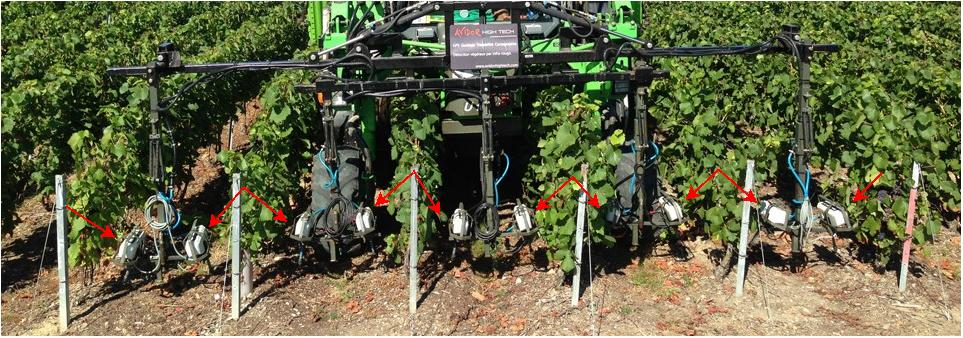
\includegraphics[width=\linewidth]{img/intro/traitement-weed-seeker}
        \caption{Présentation du WeedSeeker en viticulture}
        \label{fig:02-traitement-weed-seeker}
    \end{figure}
    
    Dans l'optique de s'affranchir des herbicides, il faut s'intéresser à des solutions alternatives de désherbage. Il existe trois grandes catégories, présentées sur la figure \ref{fig:02-traitement-alternatives}. Par exemple (a) les solutions dites mécaniques, tel-que la houe rotative, va simplement arracher les plantes émergentes. Similaires aux solutions de pulvérisation, les solutions thermiques (b) utilisent des combustibles fossiles, tel que le gaz pour brûler les adventices. Finalement, la dernière alternative (c) est le recours à l'électrique, des bandes conductrices sont appliquées au sol dans l'inter-rang. La capacité à désherber sans herbicide, permet de s'affranchir de l'apparition de résistance chez les adventices ainsi que des problèmes environnementaux liées à leur utilisation.
    
    
    \begin{figure}[H]
        \centering
        \begin{subfigure}{0.31\linewidth}
            \centering
            \source{\href{https://www.hatzenbichler.com/fr/houe-rotative}{hatzenbichler.com}}
            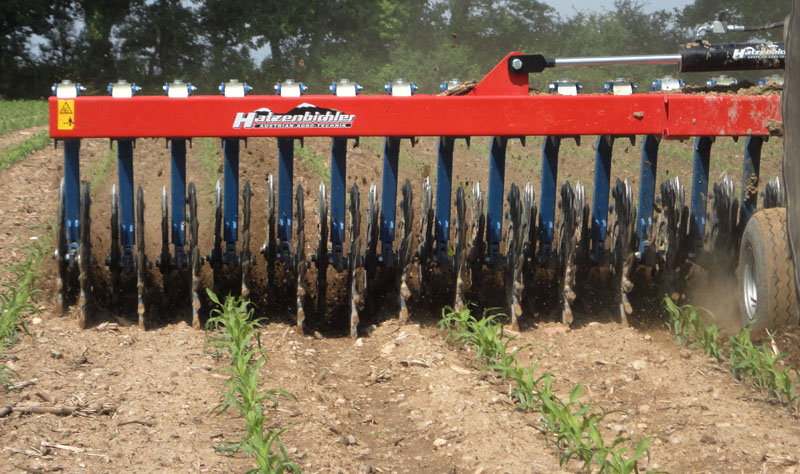
\includegraphics[width=\linewidth]{img/intro/traitement-houe-rotative}
            \caption{Houe rotative}
        \end{subfigure}
        \hfill
        \begin{subfigure}{0.31\linewidth}
            \centering
            \source{\href{https://www.annuaire-agricole.fr/fiche/2ebalm-constructeur-de-desherbeur-thermique/}{annuaire-agricole.fr}}
            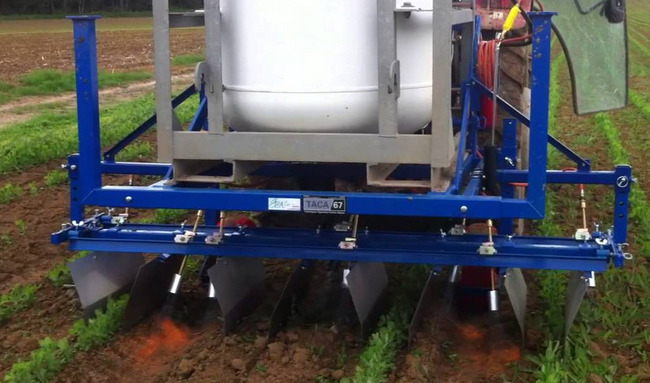
\includegraphics[width=\linewidth]{img/intro/traitement-thermique}
            \caption{Gaz}
        \end{subfigure}
        \hfill
        \begin{subfigure}{0.31\linewidth}
            \centering
            \source{\href{https://www.terre-net.fr/materiel-agricole/traitement-epandage/article/le-xpower-gen-2-arrive-chez-cnh-209-148400.html}{terre-net.fr}}
            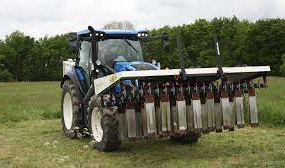
\includegraphics[width=\linewidth]{img/intro/traitement-electrique}
            \caption{Électrique}
        \end{subfigure}
        \caption{Exemples de méthodes alternatives de désherbage}
        \label{fig:02-traitement-alternatives}
    \end{figure}
    
    Actuellement, ces méthodes reposent essentiellement sur un traitement de l'inter-rang. Pour aller plus loin, les recherches actuelles, basées sur du traitement de l'image visent à détecter les plantes dans l'intra-rang. Ces méthodes sont exposées dans la section suivante.
    
    \newpage
    %\par Ces mêmes approches sont utilisées en agriculture numérique, à la différence que l'intégralité du système (Observation, Analyses, Décision) est embarqué dans une unité de calcul dédiée afin de produire en temps réel les ruptures de tronçons nécessaires. Les premières approches ont vue le jour dans les années 90, tel-que le WeedSeeker, qui détecte la présence de végétation et ouvre les électrovannes situées devant les buses lorsque c'est le cas. La limite de ce système est l'incapacité à différention une végétation type ‘culture' d'une végétation type ‘adventices ‘. Des approches plus évoluées sont en cours d'études basées sur une distinction plus fine (culture/adventice) et sont présentées dans les sections suivantes.
    
    \subsection{Les technologies de désherbage en développement}
    %\subsection{Les technologies de traitement en cours de développement}
    
    La recherche actuelle rentre davantage dans le cadre de l'agriculture numérique et les concepts sont nombreux \cite{KORRES2019243, VANMOURIK2021105031, telecom2010005}. Ainsi, une présentation exhaustive des différentes possibilités ne sera pas faite et le focus sera fait autour du Challenge ROSE. L'objectif du challenge est d'inciter à la collaboration entre équipes de recherche et industries. Ainsi différents consortiums ont été regroupés pour évaluer leurs performances respectives. Quatre consortiums ont été sélectionnés (figure \ref{fig:02-anr-challenge}).
    
    %La recherche et les concepts en agriculture numérique sont nombreux (ref ?). Ainsi une présentation exhaustive ne seras pas faite des différentes possibilités et restreindrai cette dernière au cadre du Challenge ROSE. L'objectif de ce challenge est d'inciter à la collaboration entre équipes de recherche et industries. Et s'est traduit par la constitution des consortiums de recherches engageant des collaborations entre des partenaires publics, Instituts de recherche (CNRS, Irstea, INRA, INRIA, CIRAD), Universités et établissements d'enseignement supérieur (université de Limoges, Université de Bordeaux, Montpellier Sup Agro et Bordeaux Sciences Agro), des entreprises privées du secteur agricole (Fermes Larrère, AGRIAL) et du secteur de l'agroéquipement (SITIA, CARBON BEE, Elatec, SABI AGRI), des coopératives, des chambres d'agricultures et des instituts techniques.
    
    %\begin{figure}[H]
    %	\centering
    %	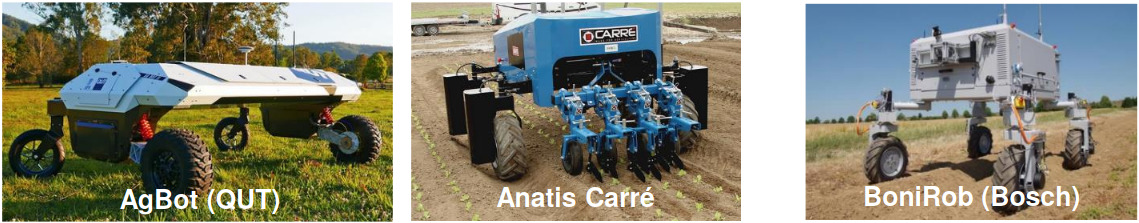
\includegraphics[width=0.7\linewidth]{img/intro/intro-binage}
    %	\caption{Binage de precision}
    %	\label{fig:02-intro-binage}
    %\end{figure}
    
    \begin{figure}[H]
        \centering
        {\scriptsize (source : challenge-rose.fr)} \\
        \includegraphics[width=1\linewidth]{img/intro/anr-difference}
        {\scriptsize De gauche a droite : BIPBIP, PEAD, Roseau et WeedElec}
        \caption{Les differents consortiums de l'ANR Challenge ROSE}
        \label{fig:02-anr-challenge}
    \end{figure}
    
    Chacun de ces consortiums propose des solutions techniques avec leurs outils respectifs (figure \ref{fig:02-anr-challenge}) dans une ou plusieurs étapes (i) détection des plantes, (ii) interprétation : culture ou adventices ? (iii) décision : faut-t-il traiter ? et (iv) action : mécanique, chimique, thermique ou électrique. Une brève présentation pour chacun d'entre eux est faite ci-dessous.
    
    \paragraph{Solution BIP BIP} : Le consortium BIP-BIP, pour Bloc-outil et Imagerie de Précision pour le Binage Intra-rang Précoce, propose \og de développer une solution mécanique pour le désherbage de cultures maraîchères et de grandes cultures au stade précoce. Cette solution repose sur un module de binage autoguidé par imagerie et télémétrie, couvrant un rang de culture. Le module s'appuie sur un système de vision fournissant la position des cultures et adventices transmise à un système décisionnel contrôlant le dispositif mécanique réalisant le binage proprement dit \fg. Le module est donc composé d'une caméra, d'une unité de calcul et d'un doigt mécanique qui est actionné au besoin en évitant les cultures. Ce dernier gratte la surface du sol permettant d'éliminer les adventices émergentes (figure \ref{fig:02-bip-bip}). % Comme on dit \og un binage vaut deux arrosages \fg
    
    \begin{figure}[H]
        \centering
        {\scriptsize (source : challenge-rose.fr)} \\
        \includegraphics[width=0.6\linewidth]{img/intro/bip-bip}
        \caption{Module de désherbage BIP-BIP}
        \label{fig:02-bip-bip}
    \end{figure}
    
    \newpage
    \paragraph{Solution PEAD} :  Ce consortium propose de gérer les tâches ``action - interprétation'' grâce à une caméra hyperspectrale spécifique développée par Carbon Bee. Des solutions de vision informatique basées sur l'intelligence artificielle ainsi que des systèmes d'imagerie hyperspectrale sont mis en œuvre. Les applications se déclinent aujourd'hui dans l'agriculture de précision permettant la détection précoce de stress et maladie dans les cultures ainsi que les adventices. La solution repose sur trois modules, une caméra, un contrôleur et un afficheur (figure \ref{fig:02-anr-pead})
    
    \begin{figure}[H]
        \centering
        {\scriptsize (source : carbonbee-agtech.fr)} \\
        \includegraphics[height=2.5cm]{img/intro/anr-pead-01} \hspace{1em}
        \includegraphics[height=2.5cm]{img/intro/anr-pead-02} \hspace{1em}
        \includegraphics[height=2.5cm]{img/intro/anr-pead-03}
        \caption{Les trois modules CarbonBee (caméra hyperspectrale, contrôleur, afficheur)}
        \label{fig:02-anr-pead}
    \end{figure}
    
    \paragraph{Solution WeedElec} : La solution WeedElec repose également sur du deep-learning pour les taches ``détection/décision''. Ils sont innovateurs sur deux aspects : (i) ils s'appuient sur de la robotique à faible consommation énergétique et légère, leur permettant d'être autonomes en énergie grâce à un panneau solaire et (ii) leurs méthodes d'action s'appuient sur des décharges électriques, une électrode est téléguidée grâce à un bras robotisé (figure \ref{fig:02-anr-weedelec}). Cette solution permet la modulation de l'intervention de manière extrêmement précise, puisque en fonction de la taille de l'adventice visée et de la force du choc électrique, l'impact sur cette dernière est différent : entre ralentissement de la croissance et brûlure.
    
    \begin{figure}[H]
        \centering
        {\scriptsize (source : challenge-rose.fr)} \\
        \includegraphics[height=2.5cm]{img/intro/anr-weedelec}
        \caption{Électrode téléguidée par le bras robotique}
        \label{fig:02-anr-weedelec}
    \end{figure}
    
    \paragraph{Solution Roseau} : Le projet ROSEAU vise à développer des outils qui interviennent sur trois composantes (perception/décision/action) via des couches de décision à plusieurs niveaux, allant du réflexe (temps-réel) aux réflexions élaborées (pouvant prendre plusieurs heures). Les différentes couches s'appuient sur des données à différentes échelles spatio-spectro-temporelles (depuis un drone et depuis un robot mobile terrestre) en provenance de caméras sensibles aux domaine du visible et de l'infrarouge. Après la prise de décision le traitement est assuré par un module spécifique, qui correspond actuellement à une roue de binage (figure \ref{fig:02-anr-roseau}). %(RObotics SEnsorimotor loops to weed AUtonomous) 
    
    \begin{figure}[H]
        \centering
        {\scriptsize (source : challenge-rose.fr)} \\
        \includegraphics[height=2.5cm]{img/intro/anr-roseau}
        \caption{Outil de binage ROSEAU}
        \label{fig:02-anr-roseau}
    \end{figure}
    
    %Le projet ROSEAU vise à développer des outils pour réaliser des opérations de désherbage sur le rang.
    %Ces outils interviennent sur 3 composantes (perception/décision/action) qui sont les 3 concepts fondamentaux des boucles sensorimotrices. Les boucles sensorimotrices sont des boucles de commande qui lient les capteurs (« sensori… ») aux actionneurs (« …motrices ») via des couches de décisions à plusieurs niveaux, allant du reflexe (boucles très rapides, de l'ordre du centième de seconde) aux réflexions élaborées (pouvant prendre plusieurs heures).
    %
    %L'objectif de ROSEAU est de décliner ce cadre aux opérations de désherbage sur le rang, avec des outils allant de la détection/éradication des adventices à la volée jusqu'à l'optimisation des itinéraires techniques en croisant les proliférations adventices et les fenêtres d'interventions.
    %\begin{itemize}
    %	\item Perception multi-échelle : depuis un drone et depuis un robot mobile terrestre
    %	\item Cameras : Utilisation de caméras sensibles aux fréquences visibles et infrarouge
    %	\item Traitements : Détection des plantes d'intérêt et des adventices via des algorithmes de traitement d'image et d'apprentissage. Volonté d'aller jusqu'à distinguer la famille d'adventice et son développement pour améliorer les décisions.
    %\end{itemize}
    
    %\begin{figure}[H]
    %	\centering
    %	\includegraphics[width=0.5\linewidth]{img/intro/anr-weedelec}
    %	\caption{Le choque electrique ralentie la croissances des adventices}
    %	\label{fig:02-anr-weedelec}
    %\end{figure}
    
    % https://www.researchgate.net/publication/341875810_Automated_Weed_Detection_Systems_A_Review
    
    \newpage
    \section{Conclusion de chapitre}
    
    %\par Comme nous l'avons vue, la connaissance des espèces et l'impacte de nos modes de production (qualité des sols, pollutions) est donc essentiel. Une relation direct et indirect entre la richesse des écosystèmes, la simplification des structures paysagères, les services écosystémiques, les pollinisateurs, la gestion des maladies, les flux de sédiments \dots, à été partiellement vue ici et démontrées récemment par \cite{Daineseeaax0121}. Ainsi tout le système et les problèmes sont liés, d'ou l'intérêt d'étudier la dynamique des systèmes, les interactions entre les éléments (figure \ref{fig:02-global-food-system}) et de préserver la biodiversité par la réduction progressive de l'usage des produits phytosanitaires. L'agriculture de précision et l'agriculture numérique sont des voies agroécologiques possibles à la réduction des conséquences de l'agriculture ``moderne''.
    
    %!Mehdi : plus de changement
    Comme nous l'avons vu, d'étroites relations existent entre les différents domaines liés à l'agriculture \cite{Daineseeaax0121} : la richesse des écosystèmes, la simplification des structures paysagères, les services écosystémiques, les pollinisateurs, la gestion des maladies, les flux de sédiments \dots . Ces liens démontrent l'importance de la connaissance des espèces, de la dynamique des systèmes, de l'interaction entre les éléments (figure \ref{fig:02-global-food-system})  et de l'impact de nos modes de production \cite{nicholson2019setting} afin d'en restreindre leurs effets néfastes \cite{Modica2016}. L'agriculture de précision et l'agriculture numérique sont des voies agroécologiques possibles à la réduction des conséquences de l'agriculture ``moderne''. 
    
    \vspace{1em}
    \begin{figure}[H]
        \centering
        \source{\cite{GODDE2021100488}}
        \includegraphics[width=0.7\linewidth]{img/intro/global-food-system-3}
        \caption{Schéma de l'interaction entre le système climatique physique, l'exposition et la vulnérabilité produisant des risques dans la chaîne de production.}
        % Le risque d'impacts liés au climat résulte de l'interaction entre les dangers liés au climat et la vulnérabilité et l'exposition des systèmes humains et naturels. Les changements dans le système climatique (à gauche) et les processus socio-économiques, y compris l'adaptation et l'atténuation (à droite), sont les moteurs des dangers, de l'exposition et de la vulnérabilité. }
        \label{fig:02-global-food-system}
    \end{figure}
    \vspace{1em}
    
    % D'autres figures
    % https://link.springer.com/article/10.1007/s11625-018-0586-x#Sec11
    % https://www.nourishlife.org/pdf/Nourish_Food_System_Map_18x24.pdf
    % https://www.researchgate.net/publication/295258838_Vulnerability_resilience_hazard_risk_damage_and_loss_A_socio-ecological_framework_for_natural_disaster_analysis
    % https://oxfordre.com/naturalhazardscience/view/10.1093/acrefore/9780199389407.001.0001/acrefore-9780199389407-e-25?mediaType=Article
    
    %! JA
    %\par Les solutions de traitement en cours de développement, repose principalement sur l'analyse d'image. Dans le cadre du Challenge RoSE, les images sont prise par un drone terrestre, visant à fournir une analyse en temps réel. A cet effet, cette thèse est divisé en plusieurs parties. Un premier chapitres est dédier aux matériels et données qui ont été acquises durant cette thèse, ainsi que les méthodes de pre-traitement qui ont été mise en œuvre. Avant de pouvoir extraire des propriété permettant leurs discrimination, il faut trouver des méthodes permettant leurs détections individuelle dans une images.
    
    Les solutions de traitement en cours de développement dans l'agriculture de précision, reposent principalement sur l'analyse d'image. Cette thèse s'inscrit dans ce domaine de par l'utilisation de méthodes d'analyses d'images classiques et de réseaux de neurones. Dans le cadre du Challenge RoSE, les images utilisées dans cette étude sont acquises par une caméra multispectrale fixée sur un drone terrestre, visant à fournir une analyse en ``temps réel''. 
    
    %À cet effet, cette thèse est divisée en plusieurs parties. Le premier chapitre est un état de l'art qui présente des méthodes d'analyse d'images. Le chapitre suivant est dédié aux matériels et aux données utilisés dans cette étude....(à demander)
    
    %Un premier chapitre est dédié aux matériels et données, ainsi que les méthodes de pré-traitement qui ont été mises en œuvre. Avant de pouvoir extraire des propriétés permettant leur discrimination, il faut trouver des méthodes permettant leur détection individuelle dans une image.
    
\end{document}